% mnras_template.tex 
%DIF LATEXDIFF DIFFERENCE FILE
%DIF DEL manuscript_v1.tex    Mon Aug  3 05:51:54 2020
%DIF ADD manuscript_rev.tex   Mon Aug  3 05:51:54 2020
%
% LaTeX template for creating an MNRAS paper
%
% v3.0 released 14 May 2015
% (version numbers match those of mnras.cls)
%
% Copyright (C) Royal Astronomical Society 2015
% Authors:
% Keith T. Smith (Royal Astronomical Society)

% Change log
%
% v3.0 May 2015
%    Renamed to match the new package name
%    Version number matches mnras.cls
%    A few minor tweaks to wording
% v1.0 September 2013
%    Beta testing only - never publicly released
%    First version: a simple (ish) template for creating an MNRAS paper

%%%%%%%%%%%%%%%%%%%%%%%%%%%%%%%%%%%%%%%%%%%%%%%%%%
% Basic setup. Most papers should leave these options alone.
\documentclass[fleqn,usenatbib]{mnras}

% MNRAS is set in Times font. If you don't have this installed (most LaTeX
% installations will be fine) or prefer the old Computer Modern fonts, comment
% out the following line
\usepackage{newtxtext,newtxmath}
% Depending on your LaTeX fonts installation, you might get better results with one of these:
%\usepackage{mathptmx}
%\usepackage{txfonts}

% Use vector fonts, so it zooms properly in on-screen viewing software
% Don't change these lines unless you know what you are doing
\usepackage[T1]{fontenc}

% Allow "Thomas van Noord" and "Simon de Laguarde" and alike to be sorted by "N" and "L" etc. in the bibliography.
% Write the name in the bibliography as "\VAN{Noord}{Van}{van} Noord, Thomas"
\DeclareRobustCommand{\VAN}[3]{#2}
\let\VANthebibliography\thebibliography
\def\thebibliography{\DeclareRobustCommand{\VAN}[3]{##3}\VANthebibliography}


%%%%% AUTHORS - PLACE YOUR OWN PACKAGES HERE %%%%%

% Only include extra packages if you really need them. Common packages are:
\usepackage{graphicx}	% Including figure files
\usepackage{amsmath}	% Advanced maths commands
\usepackage{amssymb}	% Extra maths symbols
%%%%%%%%%%%%%%%%%%%%%%%%%%%%%%%%%%%%%%%%%%%%%%%%%%

%%%%% AUTHORS - PLACE YOUR OWN COMMANDS HERE %%%%%

% Please keep new commands to a minimum, and use \newcommand not \def to avoid
% overwriting existing commands. Example:
%\newcommand{\pcm}{\,cm$^{-2}$}	% per cm-squared

%%%%%%%%%%%%%%%%%%%%%%%%%%%%%%%%%%%%%%%%%%%%%%%%%%

%%%%%%%%%%%%%%%%%%% TITLE PAGE %%%%%%%%%%%%%%%%%%%

% Title of the paper, and the short title which is used in the headers.
% Keep the title short and informative.
\title[$CO_{\mathrm{2}}$ condensation on rocky planets]{The influence of surface $CO_{\mathrm{2}}$ condensation on the evolution of warm and cold rocky planets orbiting Sun-like stars}

% The list of authors, and the short list which is used in the headers.
% If you need two or more lines of authors, add an extra line using \newauthor
\author[I. Bonati and R. Ramirez]{
I. Bonati,$^{1}$\thanks{E-mail: irene.bonati@elsi.jp (IB)}
R. M. Ramirez,$^{1,2}$
\\
% List of institutions
$^{1}$Earth-Life Science Institute, Tokyo Institute of Technology, Tokyo, Japan\\
$^{2}$Space Science Institute, Boulder, Colorado,USA\\
}

% These dates will be filled out by the publisher
\date{Accepted XXX. Received YYY; in original form ZZZ}

% Enter the current year, for the copyright statements etc.
\pubyear{2020}

% Don't change these lines
%DIF PREAMBLE EXTENSION ADDED BY LATEXDIFF
%DIF BOLD PREAMBLE %DIF PREAMBLE
\DeclareOldFontCommand{\bf}{\normalfont\bfseries}{\mathbf} %DIF PREAMBLE
\providecommand{\DIFadd}[1]{{\bf #1}} %DIF PREAMBLE
\providecommand{\DIFdel}[1]{} %DIF PREAMBLE
%DIF SAFE PREAMBLE %DIF PREAMBLE
\providecommand{\DIFaddbegin}{} %DIF PREAMBLE
\providecommand{\DIFaddend}{} %DIF PREAMBLE
\providecommand{\DIFdelbegin}{} %DIF PREAMBLE
\providecommand{\DIFdelend}{} %DIF PREAMBLE
%DIF FLOATSAFE PREAMBLE %DIF PREAMBLE
\providecommand{\DIFaddFL}[1]{\DIFadd{#1}} %DIF PREAMBLE
\providecommand{\DIFdelFL}[1]{\DIFdel{#1}} %DIF PREAMBLE
\providecommand{\DIFaddbeginFL}{} %DIF PREAMBLE
\providecommand{\DIFaddendFL}{} %DIF PREAMBLE
\providecommand{\DIFdelbeginFL}{} %DIF PREAMBLE
\providecommand{\DIFdelendFL}{} %DIF PREAMBLE
\newcommand{\DIFscaledelfig}{0.5}
%DIF HIGHLIGHTGRAPHICS PREAMBLE %DIF PREAMBLE
\RequirePackage{settobox} %DIF PREAMBLE
\RequirePackage{letltxmacro} %DIF PREAMBLE
\newsavebox{\DIFdelgraphicsbox} %DIF PREAMBLE
\newlength{\DIFdelgraphicswidth} %DIF PREAMBLE
\newlength{\DIFdelgraphicsheight} %DIF PREAMBLE
% store original definition of \includegraphics %DIF PREAMBLE
\LetLtxMacro{\DIFOincludegraphics}{\includegraphics} %DIF PREAMBLE
\newcommand{\DIFaddincludegraphics}[2][]{{\color{blue}\fbox{\DIFOincludegraphics[#1]{#2}}}} %DIF PREAMBLE
\newcommand{\DIFdelincludegraphics}[2][]{% %DIF PREAMBLE
\sbox{\DIFdelgraphicsbox}{\DIFOincludegraphics[#1]{#2}}% %DIF PREAMBLE
\settoboxwidth{\DIFdelgraphicswidth}{\DIFdelgraphicsbox} %DIF PREAMBLE
\settoboxtotalheight{\DIFdelgraphicsheight}{\DIFdelgraphicsbox} %DIF PREAMBLE
\scalebox{\DIFscaledelfig}{% %DIF PREAMBLE
\parbox[b]{\DIFdelgraphicswidth}{\usebox{\DIFdelgraphicsbox}\\[-\baselineskip] \rule{\DIFdelgraphicswidth}{0em}}\llap{\resizebox{\DIFdelgraphicswidth}{\DIFdelgraphicsheight}{% %DIF PREAMBLE
\setlength{\unitlength}{\DIFdelgraphicswidth}% %DIF PREAMBLE
\begin{picture}(1,1)% %DIF PREAMBLE
\thicklines\linethickness{2pt} %DIF PREAMBLE
{\color[rgb]{1,0,0}\put(0,0){\framebox(1,1){}}}% %DIF PREAMBLE
{\color[rgb]{1,0,0}\put(0,0){\line( 1,1){1}}}% %DIF PREAMBLE
{\color[rgb]{1,0,0}\put(0,1){\line(1,-1){1}}}% %DIF PREAMBLE
\end{picture}% %DIF PREAMBLE
}\hspace*{3pt}}} %DIF PREAMBLE
} %DIF PREAMBLE
\LetLtxMacro{\DIFOaddbegin}{\DIFaddbegin} %DIF PREAMBLE
\LetLtxMacro{\DIFOaddend}{\DIFaddend} %DIF PREAMBLE
\LetLtxMacro{\DIFOdelbegin}{\DIFdelbegin} %DIF PREAMBLE
\LetLtxMacro{\DIFOdelend}{\DIFdelend} %DIF PREAMBLE
\DeclareRobustCommand{\DIFaddbegin}{\DIFOaddbegin \let\includegraphics\DIFaddincludegraphics} %DIF PREAMBLE
\DeclareRobustCommand{\DIFaddend}{\DIFOaddend \let\includegraphics\DIFOincludegraphics} %DIF PREAMBLE
\DeclareRobustCommand{\DIFdelbegin}{\DIFOdelbegin \let\includegraphics\DIFdelincludegraphics} %DIF PREAMBLE
\DeclareRobustCommand{\DIFdelend}{\DIFOaddend \let\includegraphics\DIFOincludegraphics} %DIF PREAMBLE
\LetLtxMacro{\DIFOaddbeginFL}{\DIFaddbeginFL} %DIF PREAMBLE
\LetLtxMacro{\DIFOaddendFL}{\DIFaddendFL} %DIF PREAMBLE
\LetLtxMacro{\DIFOdelbeginFL}{\DIFdelbeginFL} %DIF PREAMBLE
\LetLtxMacro{\DIFOdelendFL}{\DIFdelendFL} %DIF PREAMBLE
\DeclareRobustCommand{\DIFaddbeginFL}{\DIFOaddbeginFL \let\includegraphics\DIFaddincludegraphics} %DIF PREAMBLE
\DeclareRobustCommand{\DIFaddendFL}{\DIFOaddendFL \let\includegraphics\DIFOincludegraphics} %DIF PREAMBLE
\DeclareRobustCommand{\DIFdelbeginFL}{\DIFOdelbeginFL \let\includegraphics\DIFdelincludegraphics} %DIF PREAMBLE
\DeclareRobustCommand{\DIFdelendFL}{\DIFOaddendFL \let\includegraphics\DIFOincludegraphics} %DIF PREAMBLE
%DIF END PREAMBLE EXTENSION ADDED BY LATEXDIFF

\begin{document}
\definecolor{greenblue}{RGB}{0,127,127}
\definecolor{greenish}{RGB}{104, 159, 56}
\newcommand{\add}[1]{\textcolor{greenblue}{#1}}
\newcommand{\irene}[1]{\textcolor{greenblue}{\textit{(Irene: #1)}}}
\newcommand{\ramses}[1]{\textcolor{greenish}{\textit{(Ramses: #1)}}}
\newcommand{\todo}[1]{\textcolor{red}{#1}}
\newcommand{\textb}[1]{\textcolor{greenblue}{#1}}
\newcommand{\textg}[1]{\textcolor{greenish}{#1}}
\label{firstpage}
\pagerange{\pageref{firstpage}--\pageref{lastpage}}
\maketitle

% Abstract of the paper
\begin{abstract}
% The abstract should briefly describe the aims, methods, and main results of the paper.
% It should be a single paragraph not more than 250 words (200 words for Letters).
% No references should appear in the abstract.
The habitable zone is the region around a star where standing bodies of liquid water \DIFdelbegin \DIFdel{are }\DIFdelend \DIFaddbegin \DIFadd{can be }\DIFaddend stable on a planetary surface. Its width is \DIFaddbegin \DIFadd{often assumed to be }\DIFaddend dictated by the efficiency of the carbonate-silicate cycle, which has maintained habitable surface conditions on our planet for billions of years. This cycle may be \DIFdelbegin \DIFdel{severely inhibited by significant }\DIFdelend \DIFaddbegin \DIFadd{inhibited by }\DIFaddend surface condensation of \DIFaddbegin \DIFadd{significant amounts of }\DIFaddend $CO_{\mathrm{2}}$ ice, which is likely to occur on distant planets containing high enough levels of atmospheric $CO_{\mathrm{2}}$. Such a process could permanently trap $CO_{\mathrm{2}}$ ice within the planet, diminishing its long-term habitability. Recent work has modeled this scenario for initially cold and icy planetary bodies orbiting our Sun. Here, we use an advanced energy balance model to consider both initially warm and cold rapidly-rotating planets orbiting F - K stars. We show that the range of orbital distances where significant surface $CO_{\mathrm{2}}$ ice condensation occurs is significantly reduced for warm start planets. Star type does not affect this conclusion, although surface $CO_{\mathrm{2}}$ ice condenses over a larger fraction of the habitable zone around hotter stars. Our warm start simulations are thus consistent with 1-D model predictions, suggesting that the \DIFdelbegin \DIFdel{size of the classical $CO_{\mathrm{2}}$-$H_{\mathrm{2}}O$ habitable zone }\DIFdelend \DIFaddbegin \DIFadd{classical habitable zone limits }\DIFaddend in those earlier models are still valid. We also find that our cold start simulations exhibit trends that are consistent with those of previous work \DIFaddbegin \DIFadd{for the Sun although we now extend the analysis to other star types}\DIFaddend .    
\end{abstract}

%DIF <  Select between one and six entries from the list of approved keywords.
%DIF <  Don't make up new ones.
\begin{keywords}
planets and satellites: terrestrial planets -- planets and satellites:atmosphere -- planets and satellites: physical evolution
\end{keywords}

%%%%%%%%%%%%%%%%%%%%%%%%%%%%%%%%%%%%%%%%%%%%%%%%%%

%%%%%%%%%%%%%%%%% BODY OF PAPER %%%%%%%%%%%%%%%%%%

\section{Introduction}

During the course of its evolution, Earth is thought to have exhibited mostly warm surface conditions that were temporarily interrupted by a few sporadic cooling episodes, triggered by processes taking place in its interior, atmosphere, and host star. The resultant climatic changes can manifest as mild oscillations, or even as extreme snowball events \DIFdelbegin \DIFdel{\citep{kirschvink1992,Hoffman1342}, with Earth’s surface being completely covered in ice }\DIFdelend \DIFaddbegin \DIFadd{capable of engulfing Earth's entire surface in ice \citep{kirschvink1992,Hoffman1342}}\DIFaddend . Nevertheless, the carbonate-silicate cycle, which maintains the balance of atmospheric $CO_{\mathrm{2}}$ between the atmosphere and the interior, has allowed Earth to escape permanent glaciation and maintain clement surface conditions throughout time \citep{Hoffman1342}.

However, large amounts of atmospheric $CO_{\mathrm{2}}$ on a cold enough planet, like is the case for some depictions of early Mars \citep{Kasting1991,wordsworth2013}, can have a detrimental effect on its habitability. A number of recent studies \DIFdelbegin \DIFdel{\citep{Kasting1991,Phumbert2005,Phumbert2011, Soto2015, Turbet2017} }\DIFdelend \DIFaddbegin \DIFadd{\citep{Kasting1991,Phumbert2005,Phumbert2011, forget2013,Soto2015, Turbet2017,kadoya_outer_2019} }\DIFaddend have shown that once $CO_{\mathrm{2}}$ partial pressures exceed the saturation level, and \DIFaddbegin \DIFadd{surface }\DIFaddend temperatures are low enough, significant condensation \DIFdelbegin \DIFdel{occurs }\DIFdelend \DIFaddbegin \DIFadd{of $CO_{\rm 2}$ ice can occur }\DIFaddend at the poles \DIFdelbegin \DIFdel{, triggering collapse }\DIFdelend (Figure~\ref{fig:Sketch}). The relatively high Rayleigh scattering of $CO_{\mathrm{2}}$, \DIFdelbegin \DIFdel{and }\DIFdelend \DIFaddbegin \DIFadd{along with }\DIFaddend the resultant increase in the planetary albedo, \DIFdelbegin \DIFdel{further }\DIFdelend \DIFaddbegin \DIFadd{work to }\DIFaddend enhance the ice-albedo feedback \citep{Kasting1991} and keep the planet cold. Moreover, the high density of $CO_{\mathrm{2}}$ ice with respect to water ice can lead to \DIFaddbegin \DIFadd{surface condensation and }\DIFaddend subsurface sequestration of the former, removing \DIFdelbegin \DIFdel{it }\DIFdelend \DIFaddbegin \DIFadd{some $CO_{\mathrm{2}}$ }\DIFaddend from the atmosphere forever\DIFdelbegin \DIFdel{, resulting in a permanent stateof glaciation. Such a scenario potentially removes or greatly mitigates the role }\DIFdelend \DIFaddbegin \DIFadd{. This could result in a permanently glaciated state. Thus, a decrease in atmospheric $CO_{\rm 2}$  can prevent planets from achieving warm states. In that case,  the influence }\DIFaddend of the carbonate-silicate cycle in sustaining \DIFdelbegin \DIFdel{habitable surface conditions }\DIFdelend \DIFaddbegin \DIFadd{habitability is greatly lessened if not gone altogether }\DIFaddend \citep{Turbet2017}.  

\DIFdelbegin \DIFdel{Thus, while }\DIFdelend \DIFaddbegin \DIFadd{While }\DIFaddend the carbonate-silicate cycle has stabilized surface temperatures over time on Earth, this might not be the case for bodies orbiting other stars and/or located at different orbital distances, and having different atmospheric $CO_{\mathrm{2}}$ inventories. In particular, $CO_{\mathrm{2}}$ pressures at large orbital distances are high enough for surface condensation and Rayleigh scattering to counter the greenhouse effect, directly impacting the width of the classical $CO_{\mathrm{2}}$-$H_{\mathrm{2}}O$ habitable zone \citep{kasting1993,KumarKopparapu2013, Ramirez2018}. 

It is therefore important to assess the role of $CO_{\mathrm{2}}$ in determining a given planet's fate. \citet{Turbet2017} have recently addressed this issue by using a 3-D Global Climate Model (GCM) to simulate the evolution of terrestrial planets across the habitable zone, and concluded that bodies \DIFdelbegin \DIFdel{remained fully frozen and exhibited }\DIFdelend \DIFaddbegin \DIFadd{initially assumed to be fully frozen remained that way, exhibiting }\DIFaddend permanent surface $CO_{\mathrm{2}}$ ice condensation at orbital distances as small as \textasciitilde $1.27$~AU from the Sun for an atmospheric $CO_{\mathrm{2}}$ pressure of $1$~bar. In comparison, 1-D calculations suggest that \DIFdelbegin \DIFdel{planets can remain habitable up }\DIFdelend \DIFaddbegin \DIFadd{the habitable zone extends }\DIFaddend to \textasciitilde $1.47$~AU at that $CO_{\mathrm{2}}$ pressure level \citep{kasting1993,KumarKopparapu2013, Ramirez2018}. 
All of this suggests that $CO_{\mathrm{2}}$ condensation in more advanced climate modeling simulations may have an even more detrimental effect on planetary habitability than previously calculated, possibly decreasing the size of the habitable zone as \DIFdelbegin \DIFdel{computed in }\DIFdelend \DIFaddbegin \DIFadd{compared to }\DIFaddend 1-D \DIFdelbegin \DIFdel{models.
%DIF < The model developed by \citet{Turbet2017} thus implies a less distant outer edge of the habitable zone compared to previous estimates \citep{KumarKopparapu2013}. 
}\DIFdelend \DIFaddbegin \DIFadd{modeling simulations.
}\DIFaddend 

\DIFdelbegin \DIFdel{However, }\DIFdelend \citet{Turbet2017} had simulated planets with initially fully-glaciated surface conditions (cold start worlds) orbiting our Sun. In contrast, habitable zone planets that start their evolution warm (warm start worlds) may exhibit \DIFdelbegin \DIFdel{different responses }\DIFdelend \DIFaddbegin \DIFadd{a different response }\DIFaddend to $CO_{\mathrm{2}}$ condensation. Here, we employ an advanced energy balance model (EBM) to investigate the parameter space of surface $CO_{\mathrm{2}}$ condensation for cold and warm rotating planets with different atmospheric $CO_{\mathrm{2}}$ pressures orbiting Sun-like (F - K) stars. We compare the cold and warm start results and discuss the implications for the width of the habitable zone.

\begin{figure}
	\includegraphics[width=0.83\columnwidth]{Figures/Sketch_idea.pdf}
    \caption{Schematic representation showing the $CO_{\mathrm{2}}$ sublimation and the polar surface temperature curves as a function of surface temperature and pressure. At the poles, the surface temperature is low enough to drop below the $CO_{\mathrm{2}}$ sublimation temperature. The presence of a sufficiently high amount of atmospheric $CO_{\mathrm{2}}$ can, in turn, drive precipitation of $CO_{\mathrm{2}}$ ice onto the planetary surface. 
    %DIF < A sufficiently high amount of atmospheric $CO_{\mathrm{2}}$ can cause the surface temperature at the poles to fall below the $CO_{\mathrm{2}}$ sublimation temperature. This, in turn, would drive precipitation of $CO_{\mathrm{2}}$ ice onto the planetary surface. 
    Such a phenomenon \DIFdelbeginFL \DIFdelFL{does not }\DIFdelendFL \DIFaddbeginFL \DIFaddFL{is more unlikely to }\DIFaddendFL happen for \DIFdelbeginFL \DIFdelFL{low contents }\DIFdelendFL \DIFaddbeginFL \DIFaddFL{a small inventory }\DIFaddendFL of \DIFaddbeginFL \DIFaddFL{atmospheric }\DIFaddendFL $CO_{\mathrm{2}}$, or when the warming effect of $CO_{\mathrm{2}}$ starts dominating at high surface pressures. Adapted from Figure 1 of \citet{Soto2015}.}
    \label{fig:Sketch}
\end{figure}

\section{Methods}
\DIFaddbegin \label{sec:Methods}
\DIFaddend \subsection{Governing equations}
We make use of an advanced non-grey energy balance model (EBM), similar to that described in \citet{RamirezLevi2018} and \cite{ramirez2020}, which is itself based on  other similar models (see also \citet{North1979},  \citet{North1981}, \citet{Williams1997}, and \citet{vladilo2013}) to determine the presence of $CO_{\mathrm{2}}$ ice condensation and its influence on the fate of bodies orbiting Sun-like stars. We study the evolution of Earth-like planets assuming cold ($T_{\mathrm{surf}}$=230 K) or warm ($T_{\mathrm{surf}}$=280 K) starts. The EBM is coupled to a 1-D radiative-convective climate model that provides the radiative transfer calculations. For a more detailed explanation of the model, the reader is redirected to \citet{ramirez2020}. \DIFaddbegin \DIFadd{We reiterate some of the key details here.
}\DIFaddend 

The present model follows the radiative energy balance principle \citep[e.g.,][]{Williams1997}, according to which planets in thermal equilibrium radiate as much energy to space as they receive from their host star. The atmospheric-ocean energy balance is expressed as \DIFdelbegin \DIFdel{\citep[e.g.,][]{james1982,Williams1997}}\DIFdelend \DIFaddbegin \DIFadd{\citep[e.g.,][]{james1982,Williams1997,batalha2016}}\DIFaddend : 

\begin{equation}
\label{ebmeq}
    C_{\mathrm{p}} \frac{\partial T(x, t)}{\partial t}-\frac{\partial}{\partial x} D\left(1-x^{2}\right) \frac{\partial T(x, t)}{\partial x}+I-L\left (\frac{dM_{\mathrm{col,CO_{\mathrm{2}}}}}{dt}\right )=S(1-A),
\end{equation}{}

where $C_{\mathrm{p}}$ is the effective heat capacity, $T$ is the zonally averaged surface temperature, $x$ is the sine of the latitude, $t$ is time, $D$ is the heat diffusion coefficient (i.e., the latitudinal transport of heat), $I$ is the outgoing infrared flux to space, $S$ is the absorbed fraction of incident solar flux, $L$ is the latent heat flux per unit mass of $CO_{\mathrm{2}}$ (5.9 \DIFdelbegin \DIFdel{x10}\DIFdelend \DIFaddbegin \DIFadd{\ $\cdot$ 10}\DIFaddend \textsuperscript{5}J/kg; \citet{forget1998}), $M_{\mathrm{col,CO_{\mathrm{2}}}}$ is the column mass of $CO_{\mathrm{2}}$ which sublimates from or condenses onto the planetary surface, and $A$ is the albedo at the top of the atmosphere\DIFdelbegin \DIFdel{over a given time step. This equation }\DIFdelend \DIFaddbegin \DIFadd{. Equation \ref{ebmeq} }\DIFaddend is solved for every time step using a second-order finite difference scheme.

The modeled planets are Earth-sized and are subdivided into 36 \DIFdelbegin \DIFdel{$5^{\circ}$ }\DIFdelend \DIFaddbegin \DIFadd{five degree }\DIFaddend wide latitudinal belts with land and ocean coverage similar to present-day Earth (i.e., $70 \%$ oceans and $30 \%$ land). Flat topography is assumed for simplicity. Planets are in circular orbits and \DIFdelbegin \DIFdel{a }\DIFdelend \DIFaddbegin \DIFadd{the length of }\DIFaddend day is 24 hours. \DIFdelbegin \DIFdel{For the calculations}\DIFdelend \DIFaddbegin \DIFadd{As per \citet{Turbet2017}}\DIFaddend , we assume that \DIFaddbegin \DIFadd{volcanic outgassing rates at a given stellar flux are always high enough to support stable climates. Thus, our worlds do not undergo limit cycles, which lead to hypothetical oscillations between warm and cold climates for planets with low volcanic outgassing rates \citep{haqq2016limit,paradise2017,kadoya_outer_2019}. We note that the existence of limit cycles is controversial and is based on various weathering and surface albedo assumptions that may not be realistic or applicable in many circumstances \citep{ramirez2017mars,graham-a}.
}

\DIFadd{Our calculations assume that }\DIFaddend atmospheres are fully-saturated and consist of $1$~bar $N_{\mathrm{2}}$ for a range of atmospheric $CO_{\mathrm{2}}$ pressures. The thermal diffusion coefficient $D$ is calculated using the following scaling relation (with the subscript "$0$" referring to present Earth values):

\begin{equation}
\label{hdiff}
    \left(\frac{D}{D_{\mathrm{0}}}\right)=\left(\frac{p}{p_{\mathrm{0}}}\right)\left(\frac{C_{\mathrm{p}}}{C_{\mathrm{p}_{0}}}\right)\left(\frac{m_{\mathrm{0}}}{m}\right)^{2}\left(\frac{\Omega_{0}}{\Omega}\right)^{2}\left(\frac{T_{\mathrm{surf,ave}}}{T_{\mathrm{0}}}\right)^{12},
\end{equation}

where $D_{\mathrm{0}}=0.58$~Wm\textsuperscript{-2}K\textsuperscript{-1}, $C_{\mathrm{p0}}=10^{3}$~g\textsuperscript{-1}kgK\textsuperscript{-1}), $p$ is the atmospheric pressure ($p_{\mathrm{0}}=1$~bar), $m$ is the atmospheric mass ($m_{\mathrm{0}}=28$~kg), $\Omega$ is the planetary rotation rate ($\Omega_{\mathrm{0}}=7.27 \cdot 10^{\mathrm{-5}}$~rads\textsuperscript{-1}), and $T_{\mathrm{surf,ave}}$ is the annual average surface temperature ($T_{\mathrm{0}}=288$~K). A crude temperature dependence is added to this equation to simulate the importance of latent heat release and transport at high temperatures \citep{Caballero2005a,Rose2017}. The exponent $12$ on the right side of Equation~\ref{hdiff} gives the right latitudinal temperature structure when comparing our results to Figure 1 from \citet{Turbet2017}, which displays an average temperature $T_{\mathrm{surf,ave}} \sim 225$~K. Without this temperature dependence, equator-pole \DIFdelbegin \DIFdel{temperatures }\DIFdelend \DIFaddbegin \DIFadd{temperature }\DIFaddend gradients are underestimated and heat transport is overestimated at cold temperatures.

The model is able to distinguish between land, ocean, ice, and clouds. As the atmosphere warms near and above the freezing point, water clouds form, with the latitudinal cloud coverage ($c$) dictated by:
\begin{equation}
\label{cloud_coverage}
    c = \min \left ( 0.72 \log \left( \frac{F_{\mathrm{C}}}{F_{\mathrm{E}}} + 1 \right ),1 \right ).
\end{equation}
Here, $F_\mathrm{C}$ is the convective heat flux, $F_\mathrm{E}$ is the convective heat flux for the Earth at $288$~K ($\sim 90$~W/m$^2$). This equation is similar to that used in the Community Atmosphere Model (CAM) GCM \citep{xu1991, yang2014} and yields an Earth-like cloud \DIFdelbegin \DIFdel{cover ($c$) of $\sim 50 \%$ }\DIFdelend \DIFaddbegin \DIFadd{coverage $c\sim 50 \%$ }\DIFaddend at a mean surface temperature $T_{\mathrm{surf}}=288$~K. 

\DIFaddbegin \DIFadd{Our modeled $CO_{\mathrm{2}}$ clouds are non-absorbing, and thus radiatively inactive. This is consistent with recent simulations suggesting that their greenhouse effect may be very small in these dense $CO_{\mathrm{2}}$ atmospheres \citep{kitzmann2016}. Even so, our $CO_{\mathrm{2}}$ clouds still impact the planetary albedo, affecting planetary surface temperatures and $CO_{\mathrm{2}}$ precipitation. Following GCM predictions \citep{forget2013}, a cloud coverage $c=50 \%$ is assumed for $CO_{\mathrm{2}}$ clouds forming within a given latitude band. 
}

\DIFaddend For each time step, spanning about $2$ hours of a planet's evolution, the new average surface temperature is updated for every latitude belt following Equation~\ref{ebmeq}, along with the resulting $H_{\mathrm{2}}O$ and $CO_{\mathrm{2}}$ inventories in the atmosphere and surface. The model simulates the entire year, including seasons, \DIFdelbegin \DIFdel{until convergence(i. e., until }\DIFdelend \DIFaddbegin \DIFadd{using an explicit forward marching numerical scheme to achieve convergence. Such convergence is reached when }\DIFaddend the average annual surface temperature does not change by more than \textasciitilde$0.1$~K \DIFdelbegin \DIFdel{) using an explicit forward marching numerical scheme}\DIFdelend \DIFaddbegin \DIFadd{and both $CO_{\mathrm{2}}$ condensation and sublimation rates are balanced}\DIFaddend . 

To validate our model, we compute the northward heat flux for a planet with $330$\DIFaddbegin \DIFadd{~}\DIFaddend ppm $CO_{\mathrm{2}}$ (i.e., similar to present Earth) and orbiting the Sun at $1$~AU at different obliquities by using the following expression:

\begin{equation}
    \mathcal{F}_{\mathrm{\lambda}}=2 \pi R \cos \lambda F_{\mathrm{\lambda}}=2 \pi R^{2} D \cos ^{2} \lambda \frac{\partial T}{\partial x},
\end{equation}

where $\mathcal{F}_{\mathrm{\lambda}}$ is the latitudinal energy transport per unit length, $R$ is the planetary radius, $\lambda$ is the latitude (between $-90^\circ$ and $90^\circ$, and $\frac{\partial T}{\partial x}$ is the temperature gradient between different latitude belts.
The obtained flux, shown in Figure~\ref{fig:flow}, matches well with similar models used in past studies \citep[e.g.,][]{WilliamsPollard}.

\begin{figure}
	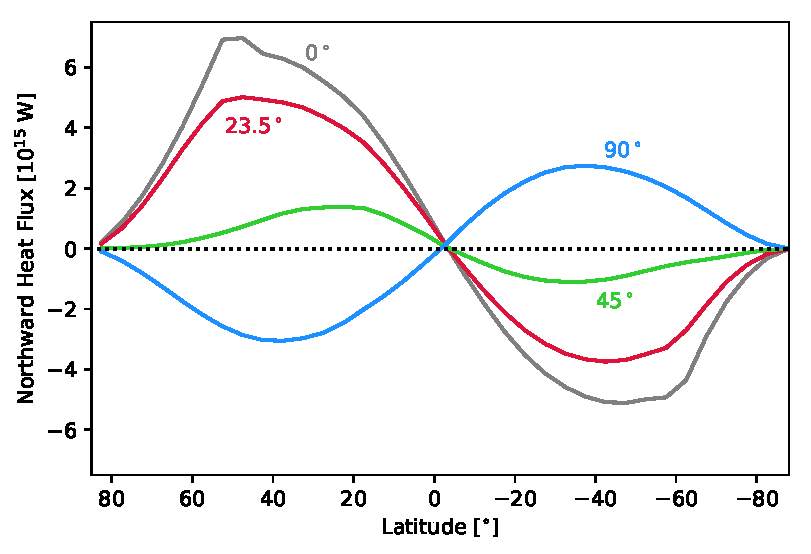
\includegraphics[width=\columnwidth]{Figures/Meridional_flow.pdf}
    \caption{Meridional heat flow for an Earth-like planet  orbiting a Sun-like star at $1$~AU, having an atmospheric pressure of $CO_{\mathrm{2}}$ of $3.3\cdot10^{-4}$~bar and obliquities $0^\circ$, $23.5^\circ$, $45^\circ$, and $90^\circ$. At low obliquities, heat is transported from the equator towards the poles, while transport in the opposite direction is favored at high enough obliquities.}
    \label{fig:flow}
\end{figure}

\DIFaddbegin \DIFadd{We also track how much surface $CO_{\mathrm{2}}$  condenses into ice, melts, or sublimates at a given latitude and time step. The phase curve of $CO_{\mathrm{2}}$ employed in this model uses established data parameterized from previous 1-D radiative-convective climate models \citep{Kasting1991} and matches very well with modern data \citep{fray_sublimation_2009}. $CO_{\rm 2}$ ice forms at cold enough surface temperatures  and when the saturation pressure is reached.  The albedo of surface $CO_{\rm 2}$ ice (dry ice) in our model is 0.6 \citet{warren_spectral_1990}, which is the same value used in \citet{Turbet2017}.
}


\DIFaddend \subsection{Initial conditions and parameter space}
We model the evolution of Earth-sized bodies, orbiting  F0, K5, and solar (\DIFdelbegin \DIFdel{a }\DIFdelend G2) stars. We vary the initial $CO_{\mathrm{2}}$ atmospheric pressure, surface temperature (cold and warm start), planetary obliquity, and semi-major axis. The initial conditions are summarized in Table~\ref{tab:ic}. If a planet starts out cold, there are \DIFaddbegin \DIFadd{initially }\DIFaddend no water clouds \DIFdelbegin \DIFdel{(initially) }\DIFdelend in the atmosphere. The global surface temperature is set to $T_{\mathrm{surf}}=230$~K, and the land snow fraction is equal to $1$ (i.e., the continents are fully covered in ice). \DIFaddbegin \DIFadd{This was done to approximate the initial conditions of \citet{Turbet2017}.
}\DIFaddend 

On the other hand, if a planet starts out warm, the surface temperature is set to $T_{\mathrm{surf}}=280$ K, with a land snow fraction of $0.5$. The fractional cloud cover from water vapor is $c_{\mathrm{H_{\mathrm{2}}O}}=0.26$ (resulting from Equation~\ref{ebmeq}). 
There are no $CO_{\mathrm{2}}$ clouds in the initial step for either case (i.e., $c_{\mathrm{CO_{\mathrm{2}}}}=0$). These starting conditions are meant to approximately simulate the modeling conditions of \citet{Turbet2017}. However, after the initial step, both cloud coverage and surface temperatures are \DIFdelbegin \DIFdel{self-consistently calculated }\DIFdelend \DIFaddbegin \DIFadd{calculated self-consistently}\DIFaddend . 

\DIFdelbegin \DIFdel{Our modeled $CO_{\mathrm{2}}$ clouds are non-absorbing, and thus radiatively inactive. This is consistent with recent simulations suggesting that their greenhouse effect may be very small in these dense $CO_{\mathrm{2}}$ atmospheres \citep{kitzmann2016}. Even so, our $CO_{\mathrm{2}}$ clouds still impact the planetary albedo, affecting planetary surface temperatures and $CO_{\mathrm{2}}$ precipitation. Following GCM predictions \citep{forget2013}, a 50 percent cloud cover is assumed for $CO_{\mathrm{2}}$ clouds forming within a given latitude band. 
}%DIFDELCMD < 

%DIFDELCMD < %%%
\DIFdelend We explore different parameters as shown in Table~\ref{tab:parameters}. We do not simulate planets located at larger semi-major axis distances than those showed in Table~\ref{tab:parameters} because modeled surface temperatures at these $CO_{\mathrm{2}}$ pressures are below what is possible for our radiative transfer model ($T_{\mathrm{surf}}=150$~K). Nevertheless, the sampled parameter space is more than sufficient to obtain the overall trends.

\begin{table}
	\centering
	\caption{Initial conditions for planets starting out cold and warm.}
	\label{tab:ic}
	\begin{tabular}{ccc} 
		\hline
		Parameter & \textbf{Cold start} & \textbf{Warm start} \\
		\hline
		Surface temperature $T_{\mathrm{surf}}$ [K] & 230 & 280 \\
		$H_{\mathrm{2}}O$ cloud fraction $c_{\mathrm{H_{\mathrm{2}}O}}$ & 0 & 0.26  \\
		$CO_{\mathrm{2}}$ cloud fraction $c_{\mathrm{CO_{\mathrm{2}}}}$ & 0 & 0 \\
		Land snow fraction & 1 & 0.5 \\
		\hline
	\end{tabular}
\end{table}

% Similarly to \citet{Turbet2017}, the $CO_{\mathrm{2}}$ clouds in our model do not absorb at any wavelengths, and thus radiatively inactive. However, even though non-absorbing, the $CO_{\mathrm{2}}$ clouds still impact the planetary albedo. Their presence therefore influences the planetary surface temperature and the precipitation of $CO_{\mathrm{2}}$.

\begin{table}
	\centering
	\caption{Parameter space investigated in the simulations.}
	\label{tab:parameters}
	\begin{tabular}{ccccc}
		\hline
		&\multicolumn{1}{c}{Parameter}&\multicolumn{3}{c}{Values}\\
		\hline
		&\multicolumn{1}{c}{$CO_{\mathrm{2}}$ partial pressure range [bar]}&\multicolumn{3}{c}{0.01-3.0}\\
		&\multicolumn{1}{c}{Obliquity [$^{\circ}$] }&\multicolumn{3}{c}{0, 23.5}\\
		&\multicolumn{1}{c}{}&\multicolumn{1}{c}{\underline{F0 star}}&\multicolumn{1}{c}{\underline{Sun}}&\multicolumn{1}{c}{\underline{K5 star}}\\
		& %DIFDELCMD < \multicolumn{1}{c}{Stellar Temperature [K]}%%%
\multicolumn{1}{c}{Stellar temperature [K]} &\multicolumn{1}{c}{7200}&\multicolumn{1}{c}{5800}&\multicolumn{1}{c}{4400}\\
		&\multicolumn{1}{c}{Stellar mass [$M_{\odot}$]}&\multicolumn{1}{c}{1.5}&\multicolumn{1}{c}{1.0}&\multicolumn{1}{c}{0.6}\\
		&\multicolumn{1}{c}{Stellar luminosity [$L_{\odot}$]}&\multicolumn{1}{c}{4.3}&\multicolumn{1}{c}{1.0}&\multicolumn{1}{c}{0.15}\\
		&\multicolumn{1}{c}{Semi-major axis range [AU]}&\multicolumn{1}{c}{2.0-3.0}&\multicolumn{1}{c}{1.0-1.5}&\multicolumn{1}{c}{0.4-0.6}\\
		\hline
	\end{tabular}
\end{table}

\section{Results}

\begin{figure*}
	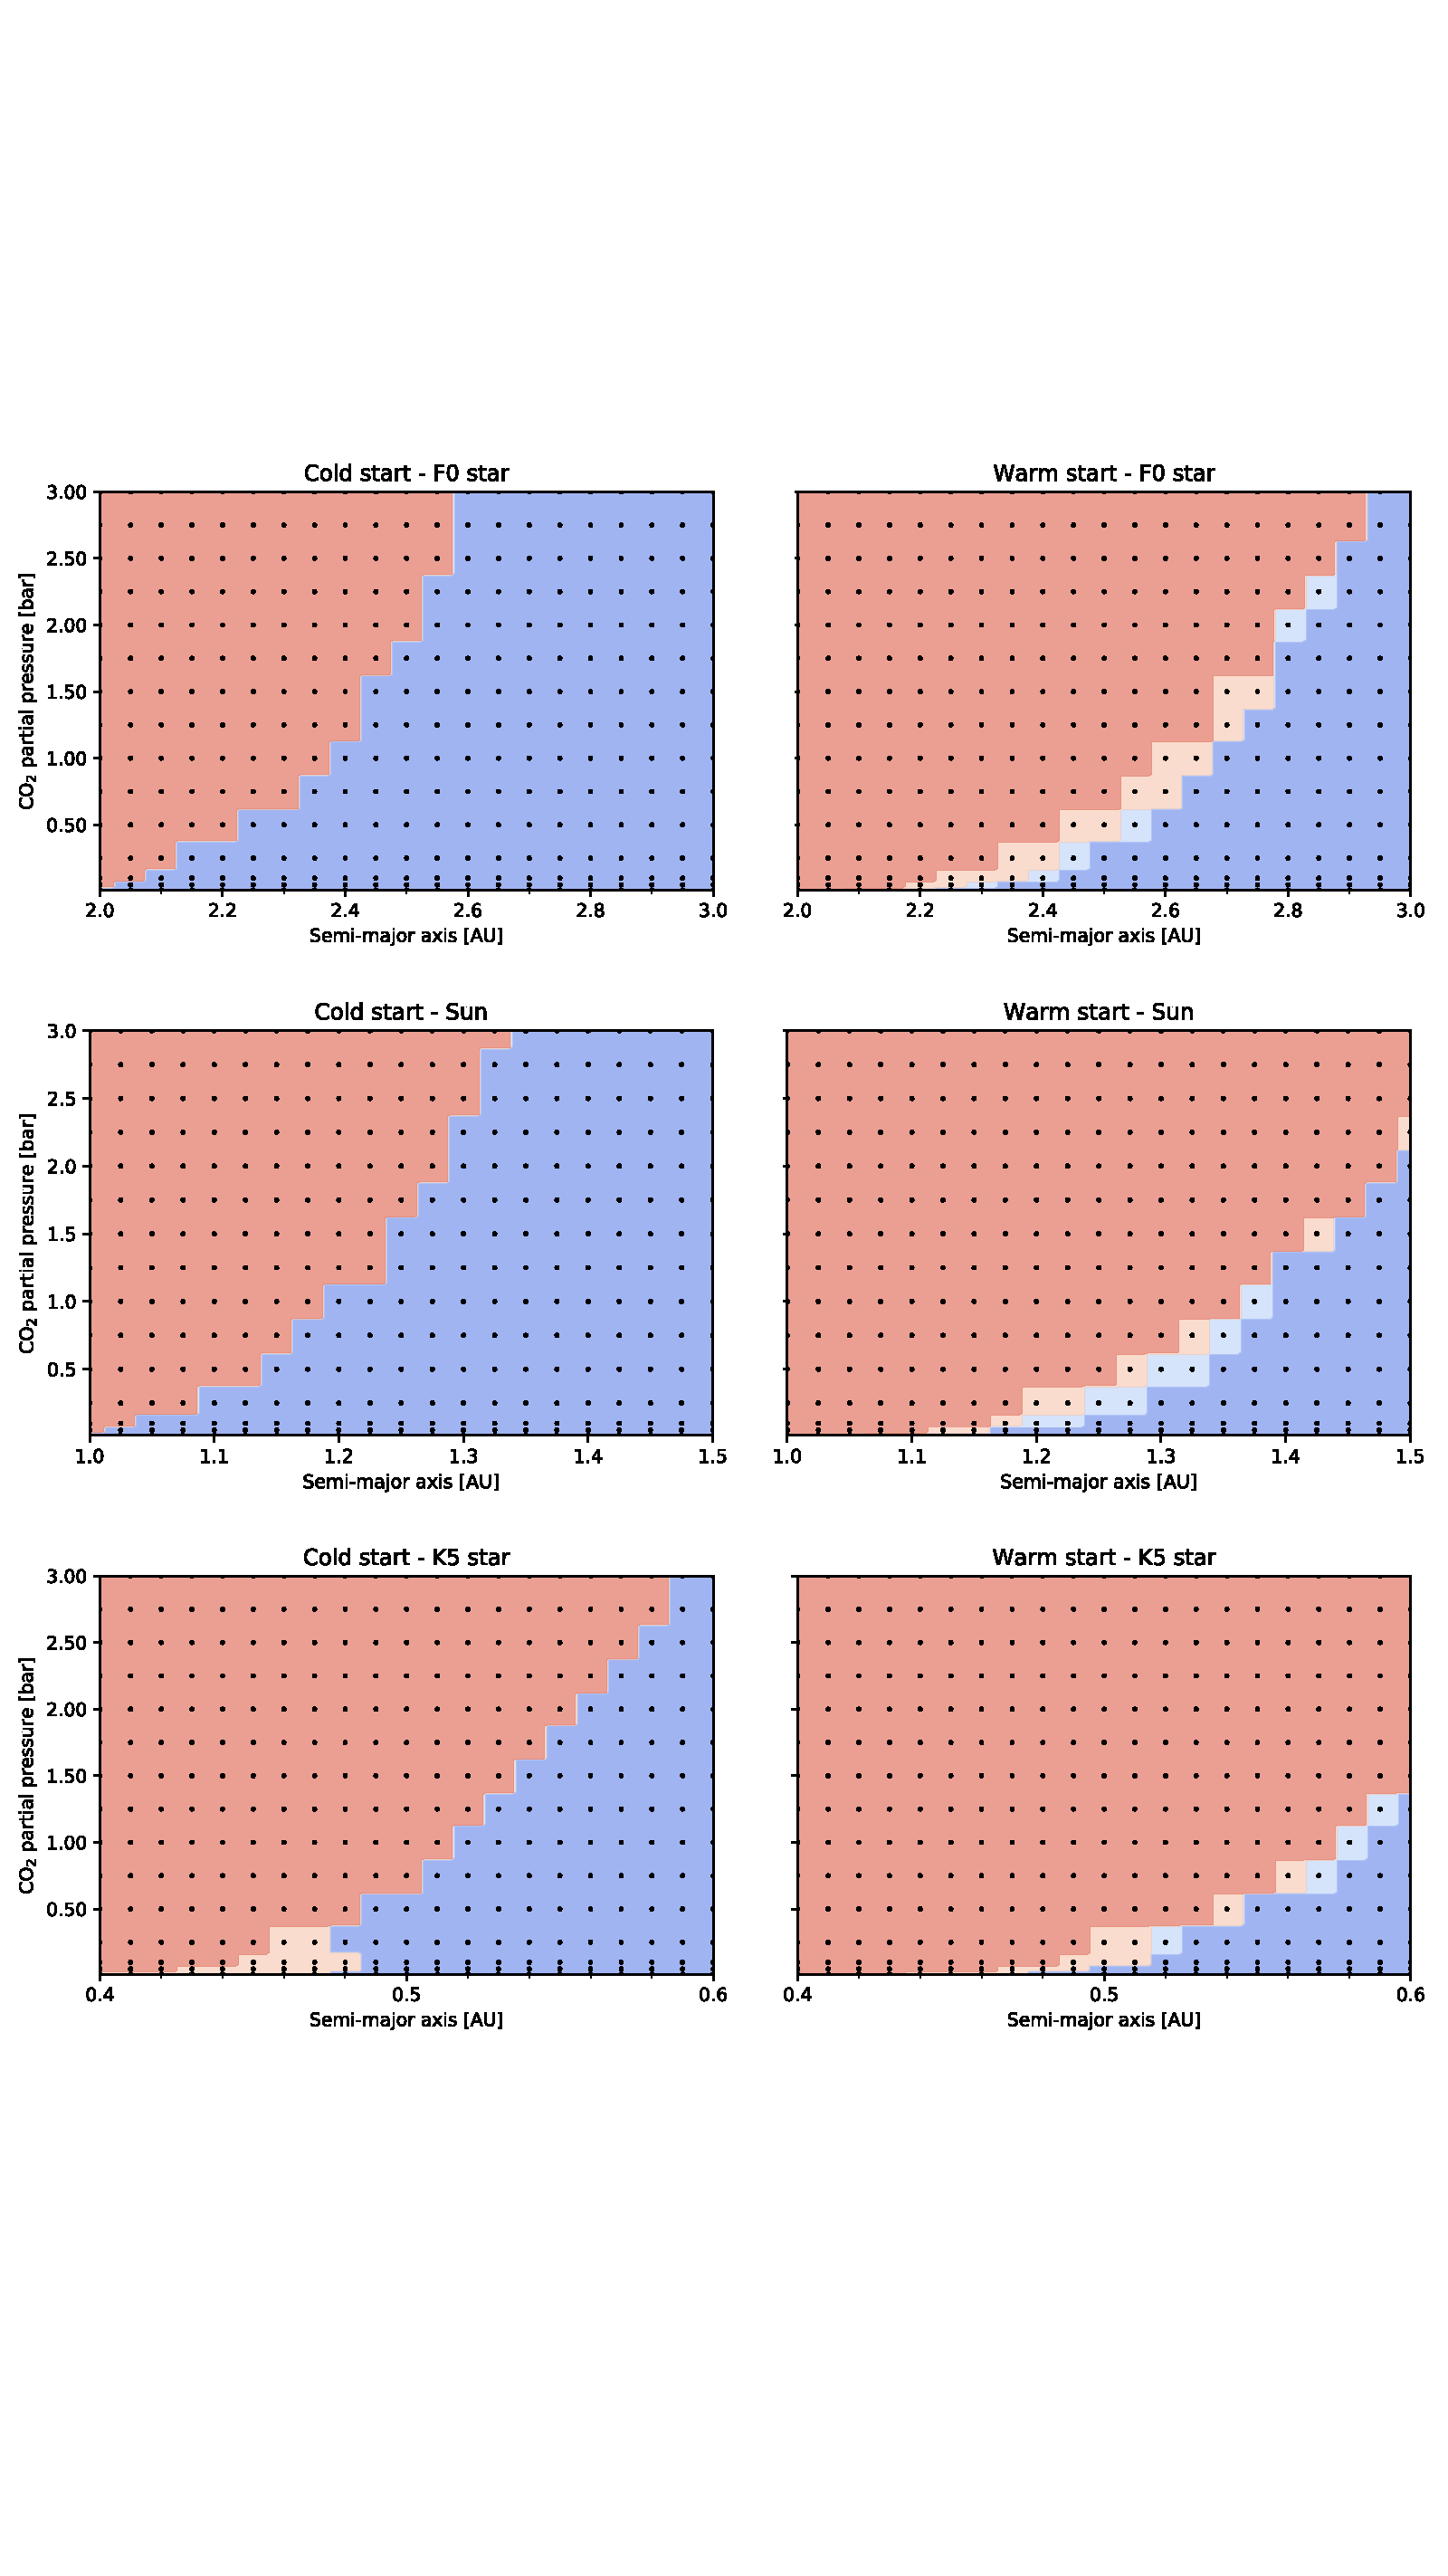
\includegraphics[width=\textwidth]{Figures/Steady_state_all.pdf}
    \caption{Steady-state solutions reached by warm \DIFaddbeginFL \DIFaddFL{(ice-free) }\DIFaddendFL and cold start (fully-glaciated body) planets orbiting F0, Sun-like and K5-type stars for a range of semi-major axes and initial partial pressures of atmospheric $CO_{\mathrm{2}}$. The modeled planets have an Earth-like continental fraction and an obliquity of $23.5^{\circ}$. The dark and light red regions comprise bodies that are ice-free and partially covered in $H_{\mathrm{2}}O$ ice, respectively. The light and dark blue regions represent partially ice-covered and snowball planets displaying permanent $CO_{\mathrm{2}}$ ice on their surfaces, respectively. Note: The horizontal scale is different for each host star. Our model predicts similar trends at $0^{\circ}$ obliquity (not shown).} 
    \label{fig:ss_all}
\end{figure*}

\begin{figure*}
	 %DIFDELCMD < 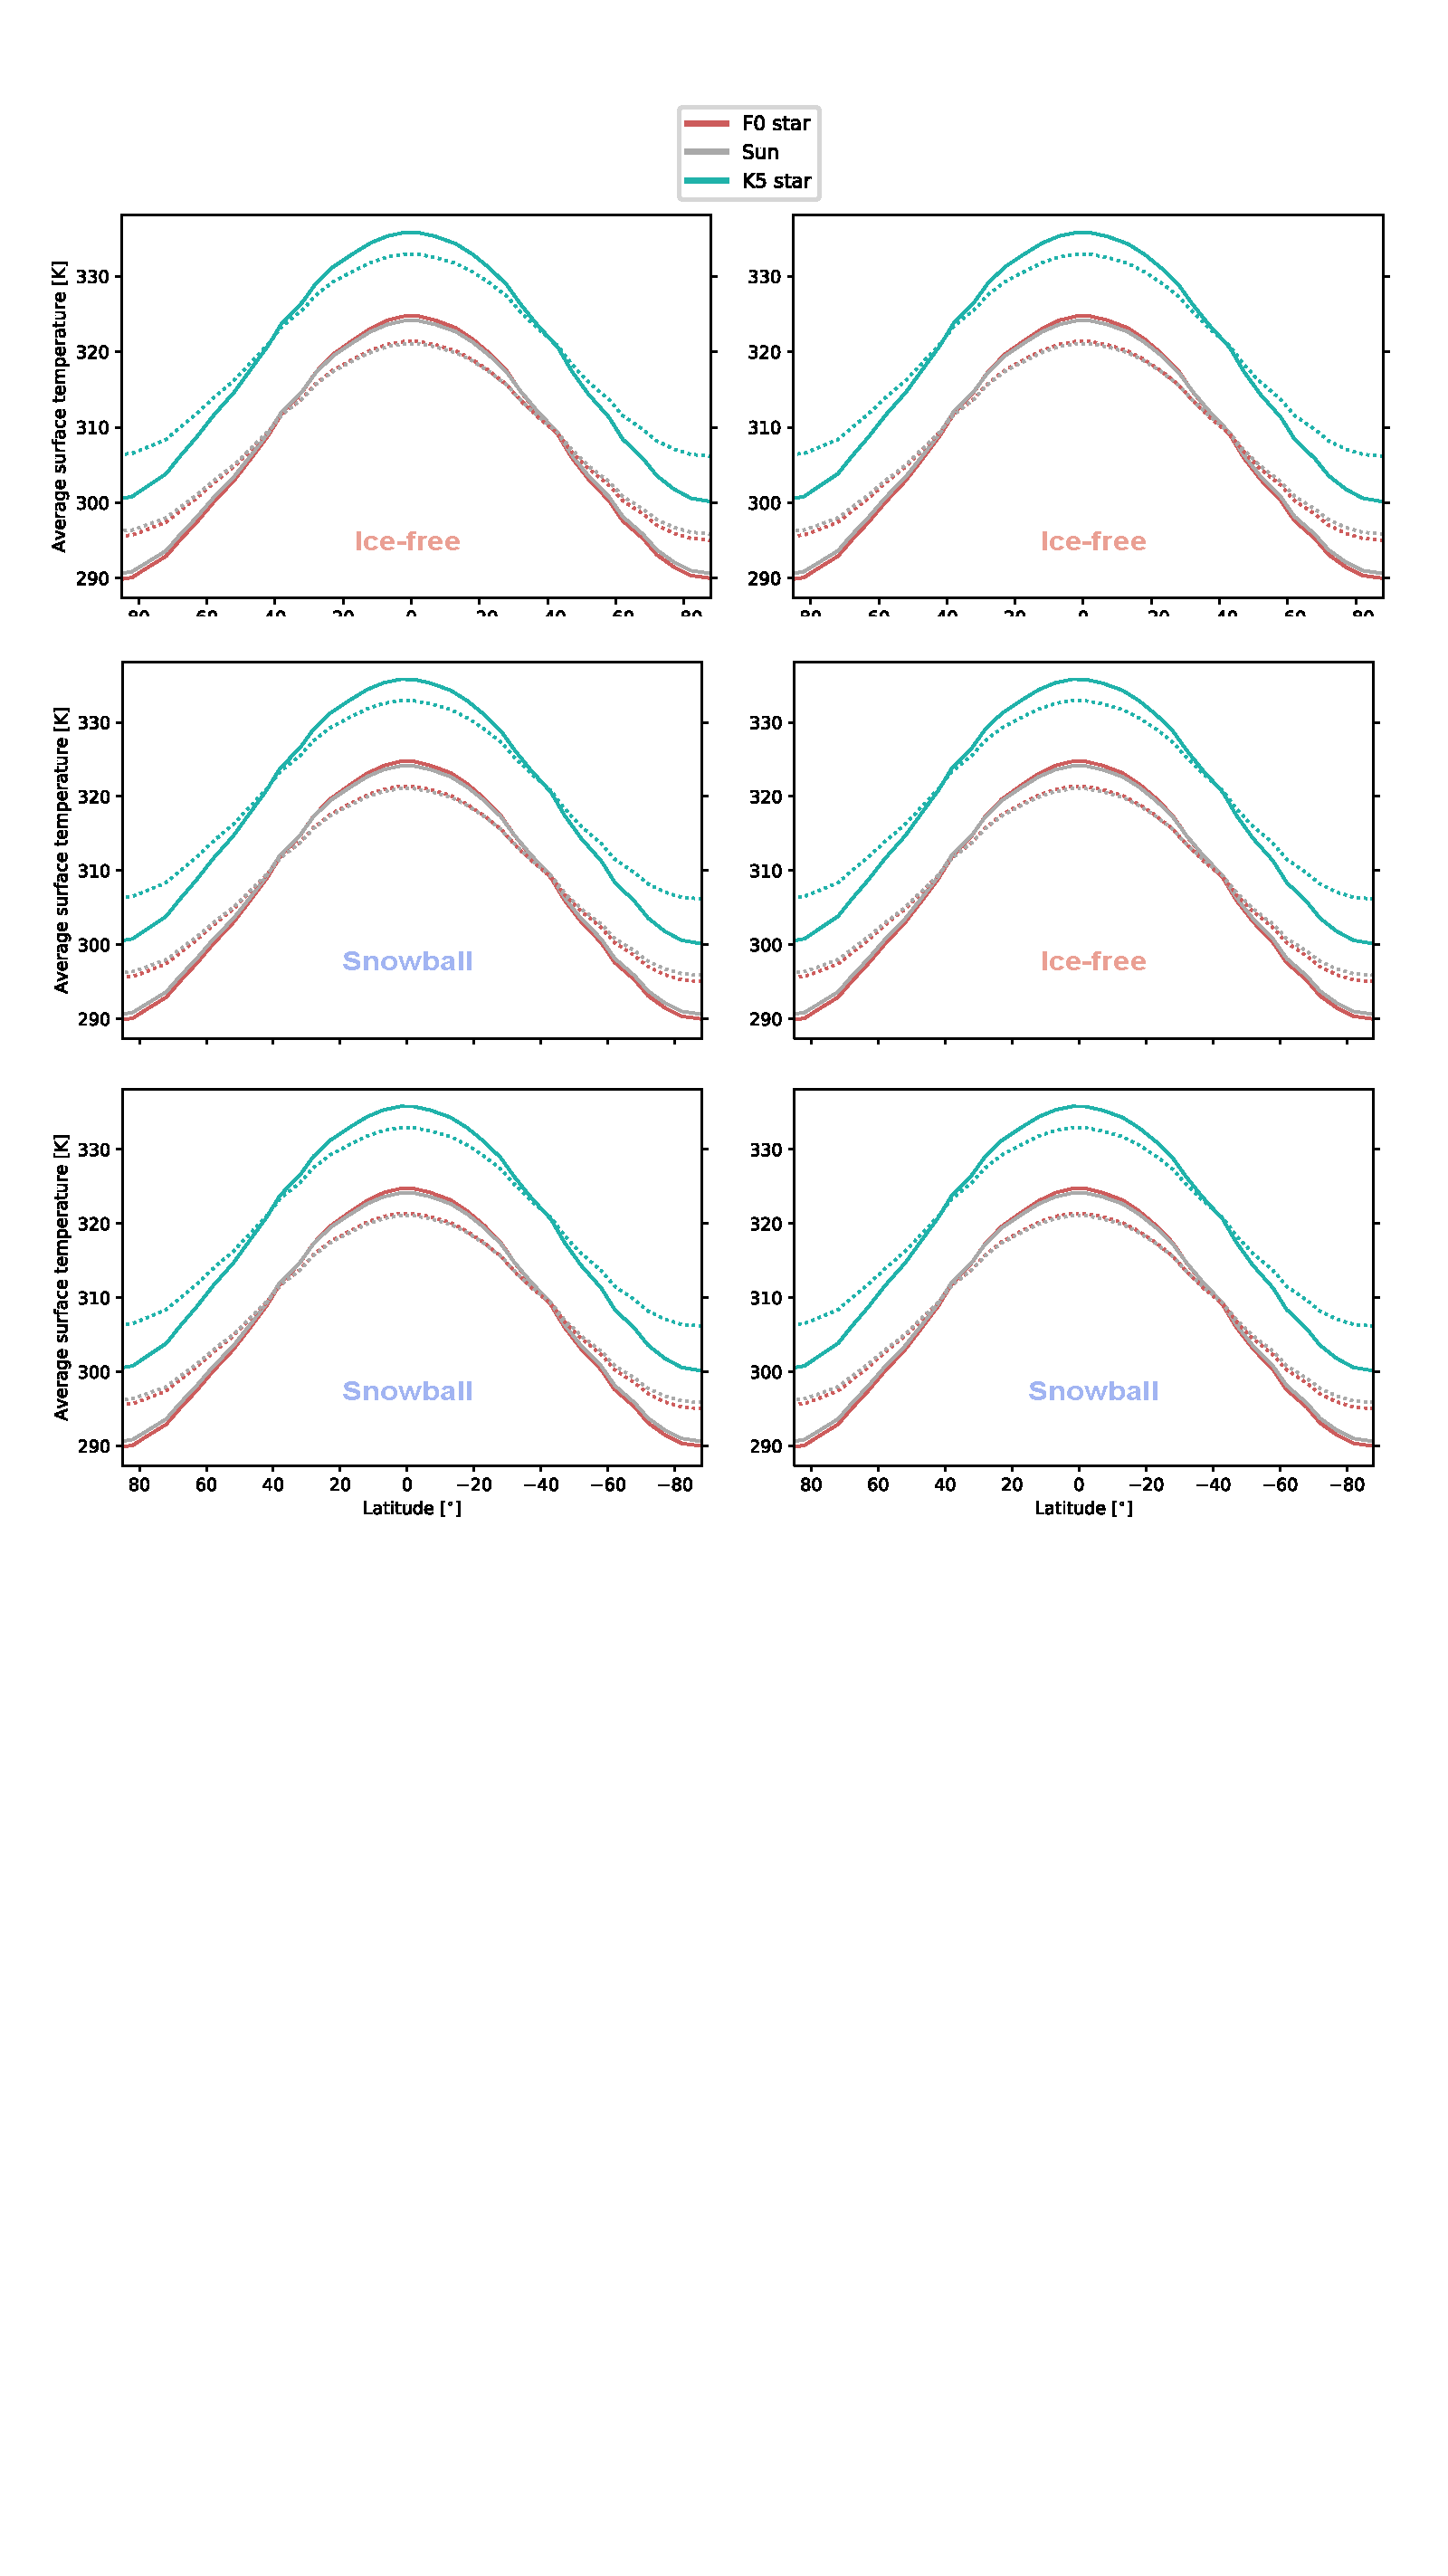
\includegraphics[width=\textwidth]{Figures/Comparison_a0.pdf}
%DIFDELCMD <     %%%
 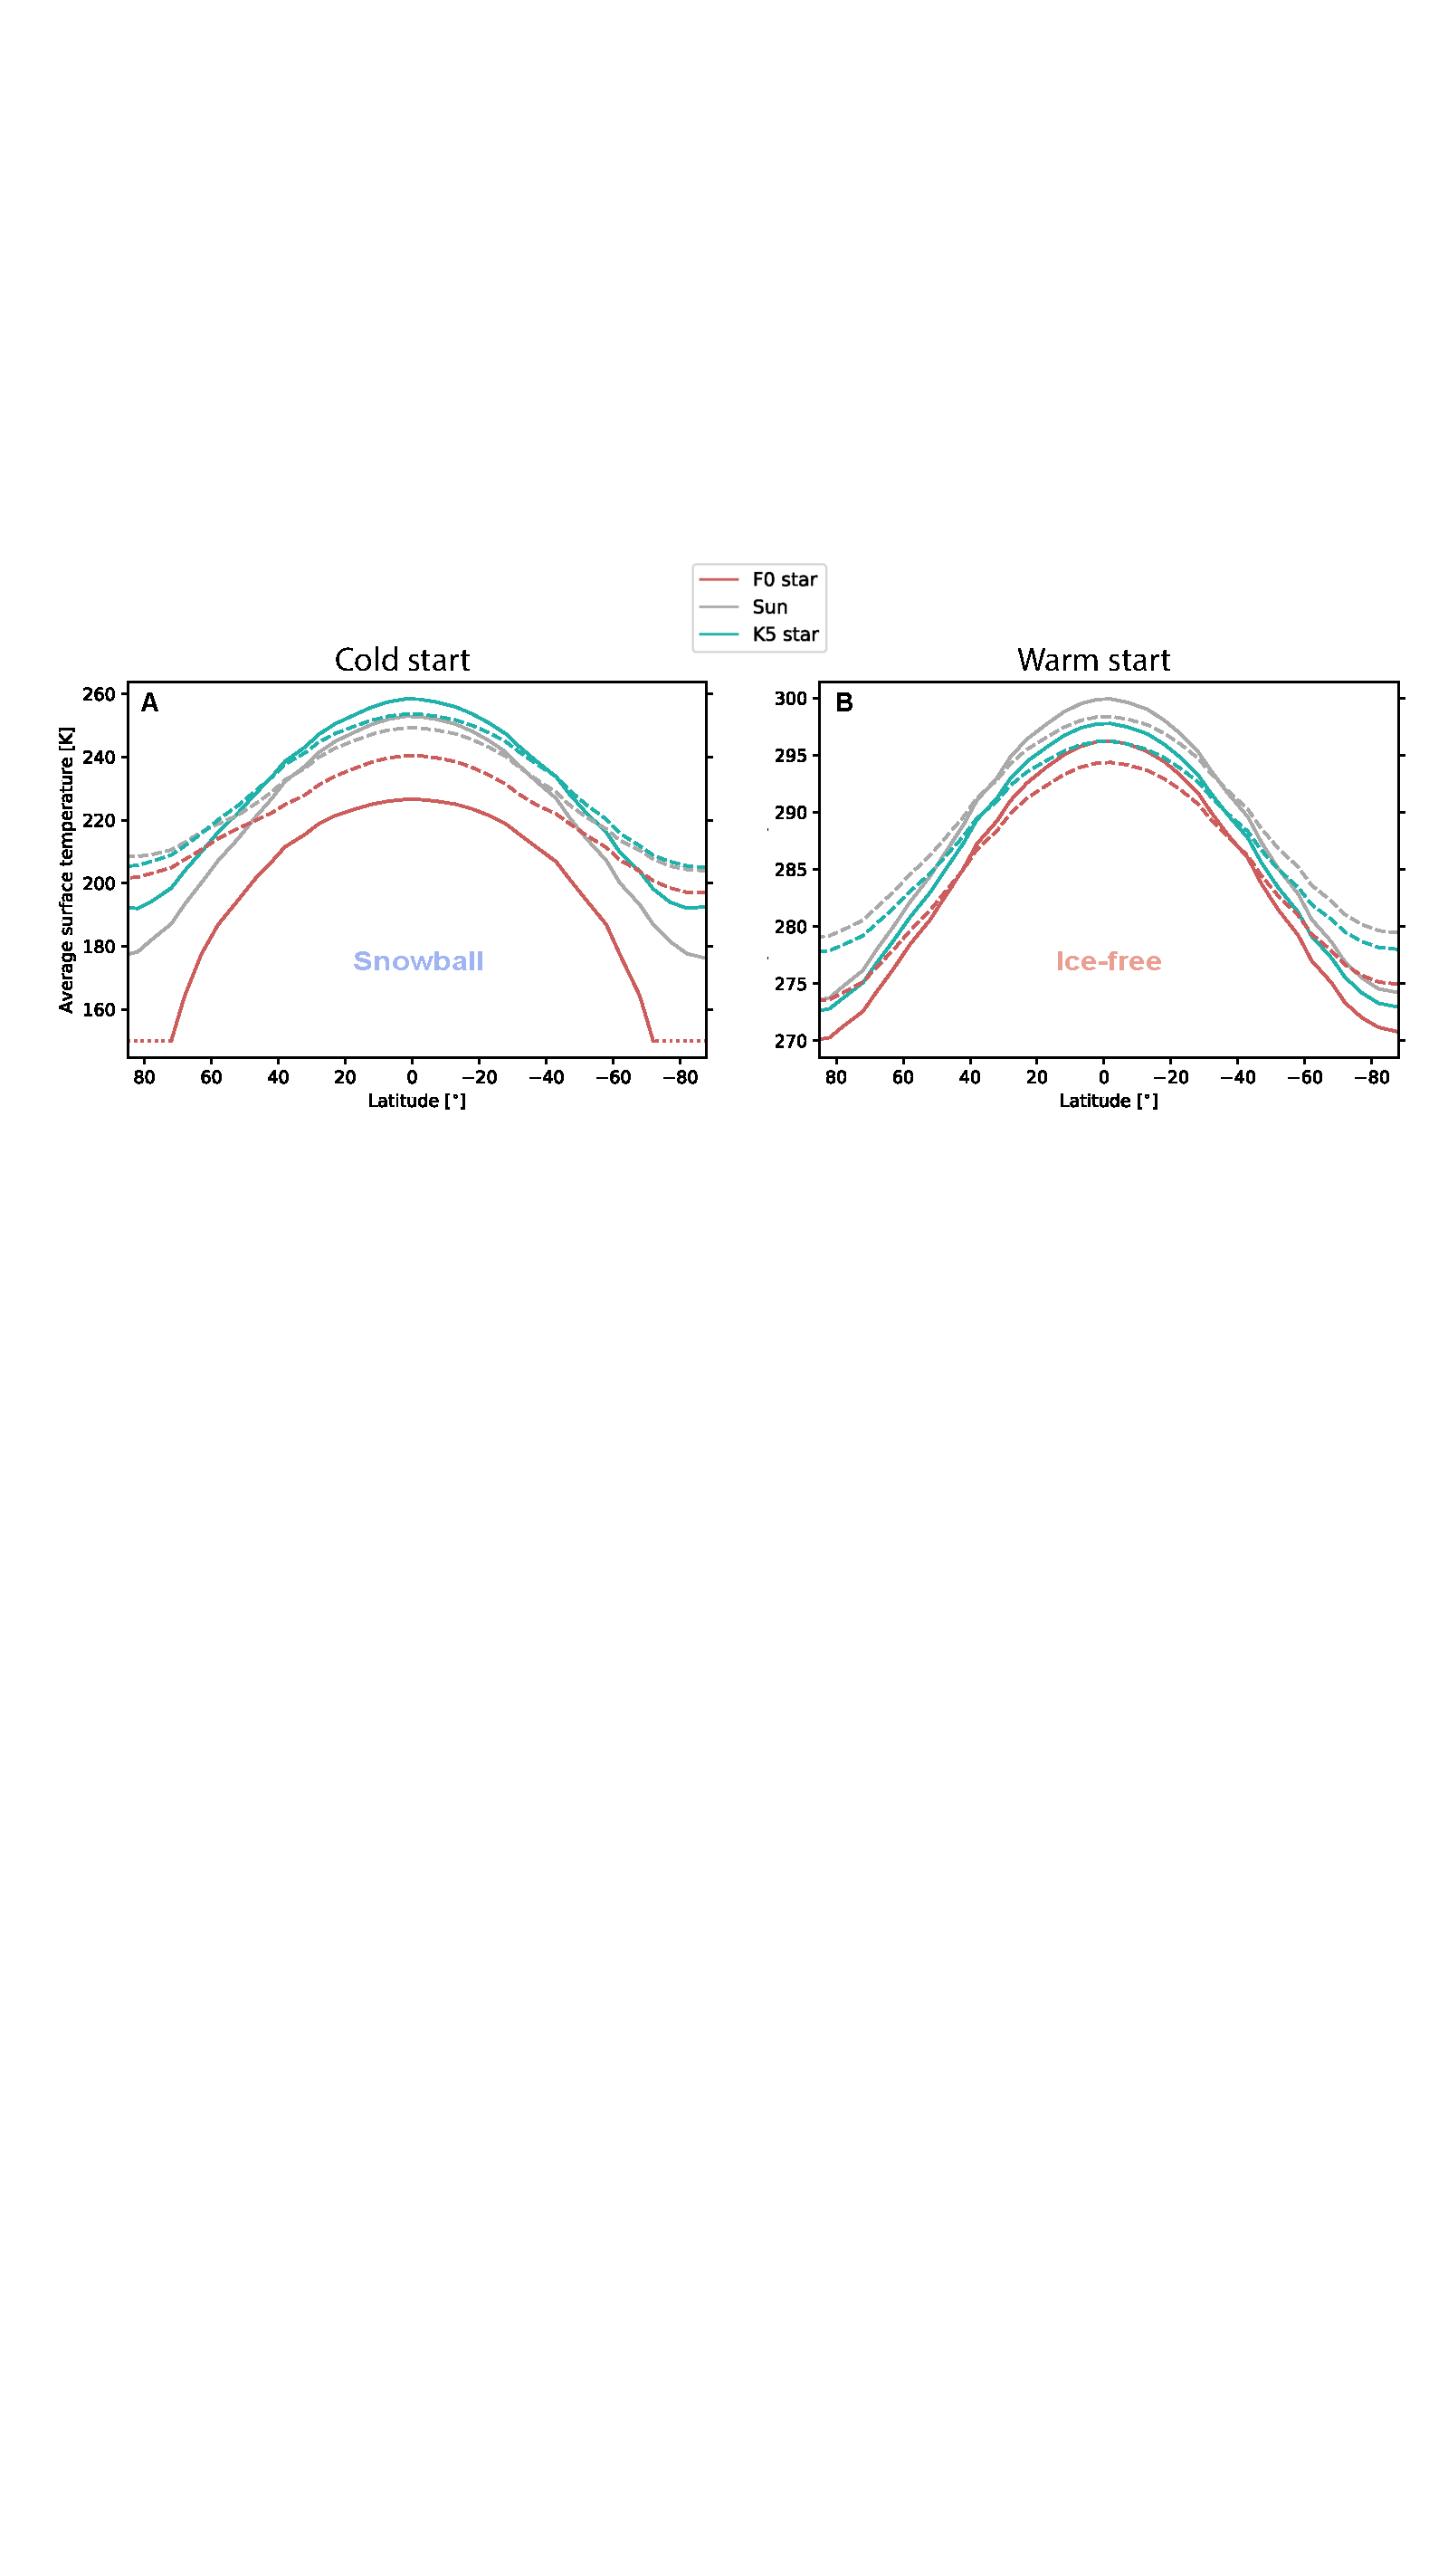
\includegraphics[width=\textwidth]{Figures/Comparison_a0_rev.pdf}
    \caption{\DIFdelbeginFL \DIFdelFL{Average }\DIFdelendFL \DIFaddbeginFL \DIFaddFL{Latitudinally averaged }\DIFaddendFL surface temperature \DIFaddbeginFL \DIFaddFL{profiles }\DIFaddendFL at the last time step \DIFdelbeginFL \DIFdelFL{as a function of latitude }\DIFdelendFL for cold start (\DIFdelbeginFL \DIFdelFL{initial  }\DIFdelendFL $T_{\mathrm{surf}}=230$~K; \DIFdelbeginFL \DIFdelFL{left column}\DIFdelendFL \DIFaddbeginFL \DIFaddFL{panel A}\DIFaddendFL ) and warm start (\DIFdelbeginFL \DIFdelFL{initial }\DIFdelendFL $T_{\mathrm{surf}}=280$~K; \DIFdelbeginFL \DIFdelFL{right column}\DIFdelendFL \DIFaddbeginFL \DIFaddFL{panel B}\DIFaddendFL ) bodies \DIFdelbeginFL \DIFdelFL{having }\DIFdelendFL \DIFaddbeginFL \DIFaddFL{located at intermediate orbital distances form their host star. Planets have }\DIFaddendFL an initial atmospheric $CO_{\mathrm{2}}$ pressure of $1$~bar \DIFdelbeginFL \DIFdelFL{. Each row samples a different region of the diagrams shown in Figure~\ref{fig:ss_all}, for planets having }\DIFdelendFL \DIFaddbeginFL \DIFaddFL{and }\DIFaddendFL obliquities of \DIFdelbeginFL \DIFdelFL{both }\DIFdelendFL $0^{\circ}$ (solid lines) and $23.5^{\circ}$ (dashed lines). The colors differentiate between planets orbiting F0, K5, and Sun-like stars at semi-major axes of \DIFdelbeginFL \DIFdelFL{$2.2$}\DIFdelendFL \DIFaddbeginFL \DIFaddFL{$2.5$}\DIFaddendFL ~AU (F0 star), \DIFdelbeginFL \DIFdelFL{$1.1$}\DIFdelendFL \DIFaddbeginFL \DIFaddFL{$1.25$}\DIFaddendFL ~AU (Sun), and \DIFdelbeginFL \DIFdelFL{$0.45$}\DIFdelendFL \DIFaddbeginFL \DIFaddFL{$0.53$}\DIFaddendFL ~AU (K5 star\DIFdelbeginFL \DIFdelFL{; first row}\DIFdelendFL )\DIFdelbeginFL \DIFdelFL{, $2.4$}\DIFdelendFL \DIFaddbeginFL \DIFaddFL{. Final atmospheric $CO_{\rm 2}$ pressures are $1$}\DIFaddendFL ~\DIFdelbeginFL \DIFdelFL{AU }\DIFdelendFL \DIFaddbeginFL \DIFaddFL{bar for planets ending up ice-free }\DIFaddendFL (\DIFdelbeginFL \DIFdelFL{F0 star}\DIFdelendFL \DIFaddbeginFL \DIFaddFL{panel B}\DIFaddendFL )\DIFdelbeginFL \DIFdelFL{, $1.25$}\DIFdelendFL \DIFaddbeginFL \DIFaddFL{. For fully glaciated planets (panel A) the final average amounts of atmospheric $CO_{\rm 2}$ are $0.87$}\DIFaddendFL ~\DIFdelbeginFL \DIFdelFL{AU }\DIFdelendFL \DIFaddbeginFL \DIFaddFL{bar }\DIFaddendFL (\DIFdelbeginFL \DIFdelFL{Sun}\DIFdelendFL \DIFaddbeginFL \DIFaddFL{$0^{\circ}$}\DIFaddendFL ) \DIFdelbeginFL \DIFdelFL{, }\DIFdelendFL and \DIFdelbeginFL \DIFdelFL{$0.53$}\DIFdelendFL \DIFaddbeginFL \DIFaddFL{$0.95$}\DIFaddendFL ~\DIFdelbeginFL \DIFdelFL{AU }\DIFdelendFL \DIFaddbeginFL \DIFaddFL{bar }\DIFaddendFL (\DIFdelbeginFL \DIFdelFL{K5 star; second row}\DIFdelendFL \DIFaddbeginFL \DIFaddFL{$23.5^{\circ}$}\DIFaddendFL ) \DIFaddbeginFL \DIFaddFL{for bodies orbiting F0 stars}\DIFaddendFL , \DIFaddbeginFL \DIFaddFL{$0.96$~bar ($0^{\circ}$) }\DIFaddendFL and \DIFdelbeginFL \DIFdelFL{$2.75$}\DIFdelendFL \DIFaddbeginFL \DIFaddFL{$0.992$}\DIFaddendFL ~\DIFdelbeginFL \DIFdelFL{AU }\DIFdelendFL \DIFaddbeginFL \DIFaddFL{bar }\DIFaddendFL (\DIFdelbeginFL \DIFdelFL{F0 star}\DIFdelendFL \DIFaddbeginFL \DIFaddFL{$23.5^{\circ}$}\DIFaddendFL ) \DIFaddbeginFL \DIFaddFL{for planets orbiting Sun-like stars}\DIFaddendFL , \DIFdelbeginFL \DIFdelFL{$1.4$}\DIFdelendFL \DIFaddbeginFL \DIFaddFL{and $0.999$}\DIFaddendFL ~\DIFdelbeginFL \DIFdelFL{AU }\DIFdelendFL \DIFaddbeginFL \DIFaddFL{bar }\DIFaddendFL (\DIFdelbeginFL \DIFdelFL{Sun}\DIFdelendFL \DIFaddbeginFL \DIFaddFL{$0^{\circ}$}\DIFaddendFL ) \DIFdelbeginFL \DIFdelFL{, }\DIFdelendFL and \DIFdelbeginFL \DIFdelFL{$0.6$}\DIFdelendFL \DIFaddbeginFL \DIFaddFL{$0.996$}\DIFaddendFL ~\DIFdelbeginFL \DIFdelFL{AU }\DIFdelendFL \DIFaddbeginFL \DIFaddFL{bar }\DIFaddendFL (\DIFdelbeginFL \DIFdelFL{K5 star;third row}\DIFdelendFL \DIFaddbeginFL \DIFaddFL{$23.5^{\circ}$}\DIFaddendFL ) \DIFaddbeginFL \DIFaddFL{for planets orbiting K5 stars}\DIFaddendFL . The \DIFdelbeginFL \DIFdelFL{colored }\DIFdelendFL text in each panel \DIFdelbeginFL \DIFdelFL{indicates }\DIFdelendFL \DIFaddbeginFL \DIFaddFL{denotes }\DIFaddendFL the final \DIFaddbeginFL \DIFaddFL{converged }\DIFaddendFL state  \DIFdelbeginFL \DIFdelFL{of all bodies contained in it }\DIFdelendFL (ice-free or snowball planets \DIFaddbeginFL \DIFaddFL{with permanent surface $CO_{\mathrm 2}$ ice}\DIFaddendFL ). \DIFaddbeginFL \DIFaddFL{Any condensing $CO_{\rm 2}$ is sequestered on the surface as $CO_{\rm 2}$ ice. The model is not accurate for latitudinal temperatures below $T_{\rm surf}=150$ K (dotted) although this does not impact the results or trends in our paper.
    %DIF > Latitudinally averaged surface temperature at the last time step as a function of latitude for cold start (initial  $T_{\mathrm{surf}}=230$~K; left column) and warm start (initial $T_{\mathrm{surf}}=280$~K; right column) bodies having an initial atmospheric $CO_{\mathrm{2}}$ pressure of $1$~bar. Each row samples a different region of the diagrams shown in Figure~\ref{fig:ss_all}, for planets having obliquities of $0^{\circ}$ (solid lines) and $23.5^{\circ}$ (dashed lines). The colors differentiate between planets orbiting F0, K5, and Sun-like stars at semi-major axes of $2.2$~AU (F0 star), $1.1$~AU (Sun), and $0.45$~AU (K5 star; panels A and B), $2.4$~AU (F0 star), $1.25$~AU (Sun), and $0.53$~AU (K5 star; panels C and D), and $2.75$~AU (F0 star), $1.4$~AU (Sun), and $0.6$~AU (K5 star; panels E and F). The colored text in each panel denotes the final state of all worlds contained in it (ice-free or snowball planets). Surface temperatures at polar latitudes are dotted as the model reaches surface temperatures that are lower than $150$~K.
    }\DIFaddendFL }
    \label{fig:comp_a0}
\end{figure*}

\subsection{Steady-state climate regimes}

\DIFaddbegin \DIFadd{We allow the $CO_{\mathrm{2}}$ partial pressure to evolve until $CO_{\mathrm{2}}$ sublimation and condensation rates are balanced. }\DIFaddend Figure~\ref{fig:ss_all} shows the steady-state climate regimes obtained for initially cold and warm Earth-sized bodies \DIFdelbegin \DIFdel{with obliquity }\DIFdelend \DIFaddbegin \DIFadd{having an obliquity of }\DIFaddend $23.5^{\circ}$ \DIFaddbegin \DIFadd{and }\DIFaddend orbiting different types of stars (\DIFdelbegin \DIFdel{Sun-like}\DIFdelend \DIFaddbegin \DIFadd{solar twin-G2}\DIFaddend , as well as F0 and K5 stars), as a function of their orbital distance and \DIFdelbegin \DIFdel{the initial atmospheric pressure of }\DIFdelend \DIFaddbegin \DIFadd{initial atmospheric }\DIFaddend $CO_{\mathrm{2}}$ \DIFaddbegin \DIFadd{pressure}\DIFaddend .  We distinguish between four final scenarios: In the first one, the planet is completely ice-free (dark red areas in Figure~\ref{fig:ss_all}). In the second one, the planet is partially covered in $H_{\mathrm{2}}O$ ice (light red areas in Figure~\ref{fig:ss_all}). In the third one, the planet is partially covered in both $H_{\mathrm{2}}O$ ice and (permanent) $CO_{\mathrm{2}}$ ice at the poles (light blue areas in Figure~\ref{fig:ss_all}). In the last one, the planet is fully ice-covered and permanent $CO_{\mathrm{2}}$ ice is present on the planetary surface (blue areas in Figure~\ref{fig:ss_all}. Permanent $CO_{\mathrm{2}}$ ice forms when condensation fluxes \DIFdelbegin \DIFdel{during the winter months do not balance sublimation taking place in the summer}\DIFdelend \DIFaddbegin \DIFadd{throughout the year outpace sublimation fluxes}\DIFaddend . 

As expected, surface $CO_{\mathrm{2}}$ ice condensation occurs at smaller orbital distances for cold start planets (left panels in Figure~\ref{fig:ss_all}) \DIFaddbegin \DIFadd{as }\DIFaddend compared to bodies \DIFdelbegin \DIFdel{starting }\DIFdelend \DIFaddbegin \DIFadd{that start }\DIFaddend out warm (right panels in Figure~\ref{fig:ss_all}).
For the solar case, the $1$~bar $CO_{\mathrm{2}}$ cold start scenario exhibits surface $CO_{\mathrm{2}}$ ice condensation starting from orbital distances as small as $\sim1.2$~AU, which compares favorably to the \DIFdelbegin \DIFdel{$1.27$}\DIFdelend \DIFaddbegin \DIFadd{$\sim 1.27$}\DIFaddend ~AU value found by \citet{Turbet2017}. The equivalent distances for the F0 and K5 stars are $\sim2.4$~AU and $\sim0.52$~AU, respectively.
In contrast, surface $CO_{\mathrm{2}}$ ice condensation for warm starts does not occur until $\sim1.38$~AU for the $1$~bar $CO_{\mathrm{2}}$ solar case, almost  $0.2$~AU farther out than for the cold start scenario. At this same pressure level, $CO_{\mathrm{2}}$ surface ice starts forming at $\sim2.7$~AU and $\sim0.58$~AU for the F0 and K5 stars, respectively. This is about \DIFdelbegin \DIFdel{$0.03$}\DIFdelend \DIFaddbegin \DIFadd{$0.3$}\DIFaddend ~AU and $0.06$~AU farther out than for the equivalent cold start cases.
The distances beyond which surface $CO_{\mathrm{2}}$ ice condensation starts forming are pressure-dependent, as a result of the greenhouse effect \DIFdelbegin \DIFdel{exerted by }\DIFdelend \DIFaddbegin \DIFadd{of }\DIFaddend $CO_{\mathrm{2}}$. At higher pressures, surface $CO_{\mathrm{2}}$ ice condensation in both warm and cold start cases occurs farther away from the host star, whereas the opposite takes place at lower pressures.

Moreover, the surface $CO_{\mathrm{2}}$ ice condensation encompasses a larger region for the hotter stars (alternatively, the red region is larger for cooler stars). This is because near-infrared absorption is lower and Rayleigh scattering is higher for planetary atmospheres orbiting hotter stars, cooling the planet and causing $CO_{\mathrm{2}}$ surface ice condensation to occur closer to the star. For comparison, 1-D radiative-convective climate modeling simulations predict that planets with a $1$~bar $CO_{\mathrm{2}}$ atmosphere orbiting F0, solar, and K5 stars can remain habitable at distances as far as $\sim 2.75$, $1.47$, and $0.58$~AU, respectively \citep{kasting1993, KumarKopparapu2013,Ramirez2018}, assuming the luminosity values given in Table~\ref{tab:parameters}. These values are only slightly farther out than the most distant extent of the red regions at the $1$~bar level (Figure~\ref{fig:ss_all}). Although nearly the same size, the warm regions in the warm starts still span slightly smaller areas (generally) than predicted in 1-D radiative-convective climate modeling simulations \citep{kasting1993, KumarKopparapu2013,Ramirez2018}. This is because of the EBM's increased ice-albedo feedback.

A key observation from our cold starts is that a planet cannot escape full glaciation for orbital distances exceeding $\sim 2.55$\DIFdelbegin \DIFdel{~AU}\DIFdelend , $\sim1.33$\DIFdelbegin \DIFdel{~AU}\DIFdelend , and $\sim0.58$~AU for the F0, solar, and K5 star cold start scenarios (Figure~\ref{fig:ss_all}). In these cases, the planet remains glaciated with surface $CO_{\mathrm{2}}$ ice condensation regardless of the atmospheric $CO_{\mathrm{2}}$ content (Figure~\ref{fig:ss_all}). This difference is attributed to the weaker heat transport and higher surface albedo associated with such cold starts. Although \citet{Turbet2017} does not necessarily obtain $CO_{\mathrm{2}}$ surface ice in all of these cases, in agreement with our model, they predict snowball states. 

%DIF >  Similar to what is shown in Figure~\ref{fig:Sketch}, at high enough atmospheric $CO_{\mathrm{2}}$ pressures the greenhouse effect dominates tends to inhibit surface ice condensation. Under these conditions $CO_{\mathrm{2}}$ ice condensation becomes marginal at both obliquities, consistent with trends that were also found in previous work \citep{Soto2015}. 
\DIFaddbegin 

\DIFaddend \subsection{Latitudinal variation of surface temperature \DIFaddbegin \DIFadd{and amount of surface $CO_{\rm 2}$ ice}\DIFaddend }
\label{sec:surf_temp}
The  average surface temperature at the last time step as a function of latitude is illustrated in Figure~\ref{fig:comp_a0}, for both initially cold and warm planets having \DIFaddbegin \DIFadd{an initial atmospheric $CO_{\mathrm{2}}$ pressure of }\DIFaddend $1$~bar \DIFdelbegin \DIFdel{of $CO_{\mathrm{2}}$ in their atmospheres and obliquities }\DIFdelend \DIFaddbegin \DIFadd{and obliquity angles of }\DIFaddend $23.5^{\circ}$ \DIFaddbegin \DIFadd{(dashed lines) }\DIFaddend and $0^{\circ}$ \DIFdelbegin \DIFdel{. }\DIFdelend \DIFaddbegin \DIFadd{(solid lines). These planets are located at intermediate orbital distances from the host star, close to the transition between ice-free and fully ice-covered bodies (see Figure \ref{fig:ss_all}). At such semi-major axes (and intermediate atmospheric $CO_{\rm 2}$ pressures), the initial state of a planet (warm or cold) is a strong predictor of  the final state of the planet. For instance, such warm start planets end up warm as well. Likewise, a cold start planet at these distances converges to a frozen solution also. In contrast, at smaller  orbital distances, the intense starlight produces warm planets regardless of the starting state. At larger semi-major axes, the reduction in starlight, combined with more intense surface $CO_{\rm 2}$ condensation, favors cold solutions (Figure \ref{fig:ss_all}). 
}

\DIFaddend Low obliquity bodies receive more direct insulation at the equator, which causes large temperature differences between the latter and the poles, as well as generally lower polar surface temperatures. This also produced the tendency for equatorial surface temperatures to be higher at $0^{\circ}$ \DIFdelbegin \DIFdel{compared to }\DIFdelend \DIFaddbegin \DIFadd{than at }\DIFaddend $23.5^{\circ}$ obliquity, especially at higher $CO_{\mathrm{2}}$ pressures \DIFdelbegin \DIFdel{. This, in turn, would cause }\DIFdelend \DIFaddbegin \DIFadd{(Figure \ref{fig:comp_a0}). While this could lead to }\DIFaddend more surface $CO_{\mathrm{2}}$ ice \DIFdelbegin \DIFdel{to be }\DIFdelend \DIFaddbegin \DIFadd{being }\DIFaddend present at higher ($23.5^{\circ}$) obliquity\DIFdelbegin \DIFdel{(see Figure~\ref{fig:CO2_ice}).
%DIF <  We find that obliquity variations impact surface temperature distributions the most when the planet is not located near the boundary between the warm red and cold blue regions (Figure \ref{fig:ss_all}). In contrast, near or at these transitions, such obliquity effects are outstripped by the ice-albedo feedback. Thus, the size of the habitable zone remains relatively unaffected across the two obliquity levels.
}%DIFDELCMD < 

%DIFDELCMD < %%%
\DIFdel{We also }\DIFdelend \DIFaddbegin \DIFadd{, we }\DIFaddend find that the \DIFdelbegin \DIFdel{final state of a planet (i.e., whether it ends up being ice-free, partially ice-covered or a snowball) is not greatly influenced by obliquity variations for these dense $CO_{\mathrm{2}}$ atmospheres  that are located near or very far away from their host stars (first and last rows in Figure~\ref{fig:comp_a0}). This is because at these distances, either the ice-albedo feedback (at farther distances) or the greenhouse effect (at closer distances) outstrip the impact of obliquity variations. This trend holds true whether the planet has a cold or warm start (Figure~\ref{fig:comp_a0}). However, at intermediate orbital distances (second row in Figure ~\ref{fig:comp_a0}), close to the interface between the red and the blue regions (Figure~\ref{fig:ss_all}), obliquity variations have a bigger impact on the final state.
%DIF < 
}%DIFDELCMD < 

%DIFDELCMD < %%%
%DIF <  \begin{figure}
%DIF <  	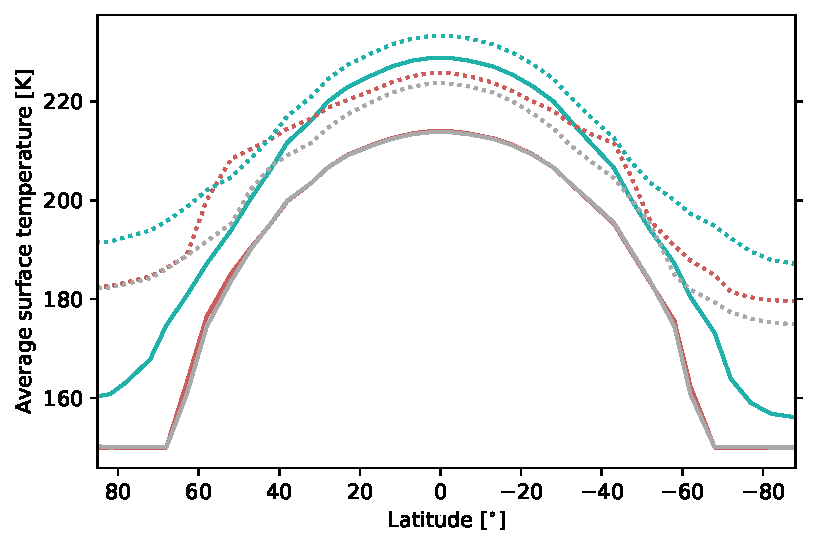
\includegraphics[width=\columnwidth]{Figures/T_ave.pdf}
%DIF <      \caption{Average surface temperature at the last time step as a function of latitude for cold start ($T_{\mathrm{surf}}=230$~K) bodies having an initial atmospheric $CO_{\mathrm{2}}$ pressure of $1$~bar and obliquities $0^{\circ}$ (solid lines) and $23.5^{\circ}$ (dashed lines), orbiting F0, K5, and Sun-like stars at distances of $2.7$, $0.6$, and $1.4$~AU, respectively.}
%DIF <      \label{fig:T_ave}
%DIF <  \end{figure}
%DIFDELCMD < 

%DIFDELCMD < %%%
\subsection{\DIFdel{Fraction of surface $CO_{\mathrm{2}}$ ice}}
%DIFAUXCMD
\addtocounter{subsection}{-1}%DIFAUXCMD
%DIFDELCMD < 

%DIFDELCMD < %%%
\DIFdel{As shown by the Mars simulations of \citet{Soto2015}, the fraction of atmospheric $CO_{\mathrm{2}}$ that condenses onto the surface depends heavily on the atmospheric $CO_{\mathrm{2}}$ pressure and the planetary obliquity. Consistent with that study, we generally find that the amount of condensed $CO_{\mathrm{2}}$ ice (i. e., }\DIFdelend \DIFaddbegin \DIFadd{portion of precipitated $CO_{\rm 2}$ is always higher for low obliquity planets having an initial atmospheric $CO_{\rm 2}$ pressure of $1$~bar (see caption in Figure \ref{fig:comp_a0}). For example, low and high obliquity planets orbiting F0 stars end up precipitating $\sim 13 \%$ and $\sim 5\%$ of atmospheric $CO_{\rm 2}$ onto the planetary surface, respectively. Conversely, obliquity variations have a smaller effect for planets orbiting cooler K5 stars, for which the surface sequestered similar amounts of atmospheric $CO_{\rm 2}$ at the two tilt angles ($\sim 0.1 \%$ at low and $\sim 0.4\%$ at high obliquity). This is because near-infrared absorption is stronger (and Rayleigh scattering is weaker) for worlds orbiting cooler stars \citep{kasting1993}. This allows for proportionately more energy to be transported across the planet, increasing }\DIFaddend the \DIFdelbegin \DIFdel{fraction of initial atmospheric $CO_{\mathrm{2}}$ that precipitates onto the planetary surface) is highest at low obliquity ($0^{\circ}$) and at low/intermediate pressures (Figure~\ref{fig:CO2_ice}). Such a trend is expected because equator-pole transport is relatively weak at low obliquities and pressures, which favors  $CO_{\mathrm{2}}$ ice condensation at the poles. 
}%DIFDELCMD < 

%DIFDELCMD < %%%
\DIFdel{At very low atmospheric $CO_{\mathrm{2}}$ pressures (i.e., smaller than $0.1$~bar), saturation is hardly ever reached, and even if the planetary surface is cold enough, $CO_{\mathrm{2}}$ will not precipitate or precipitate in very low amounts (Figure~\ref{fig:CO2_ice}) . 
%DIF < As a result, the fraction of atmospheric $CO_{\mathrm{2}}$ lost to collapse is very low, on the order of $1$~\% (Figure~\ref{fig:CO2_ice}).
Similarly, at high enough atmospheric $CO_{\mathrm{2}}$ pressures (above 2 bar) the }\DIFdelend greenhouse effect \DIFdelbegin \DIFdel{dominates and inhibits surface ice condensation, especially at lower latitudes. Under these conditions $CO_{\mathrm{2}}$ ice condensation becomes marginal (< 1 percent atmospheric $CO_{\mathrm{2}}$) at both obliquities (Figure~\ref{fig:CO2_ice}), consistent with trends that were also found in \citet{Soto2015}. 
For pressures higher than $\sim2$~bar surface $CO_{\mathrm{2}}$ condensation is slightly larger at higher ($23.5^{\circ}$) obliquity(Figure~\ref{fig:CO2_ice}).
We attribute this to slightly less efficient equator-pole transport at higher obliquity for the highest pressures.
}\DIFdelend \DIFaddbegin \DIFadd{and reducing the amount of surface $CO_{\rm 2}$ condensation, making K-star planets less sensitive to modest changes in obliquity.
}\DIFaddend 

\DIFdelbegin %DIFDELCMD < \begin{figure}
%DIFDELCMD < 	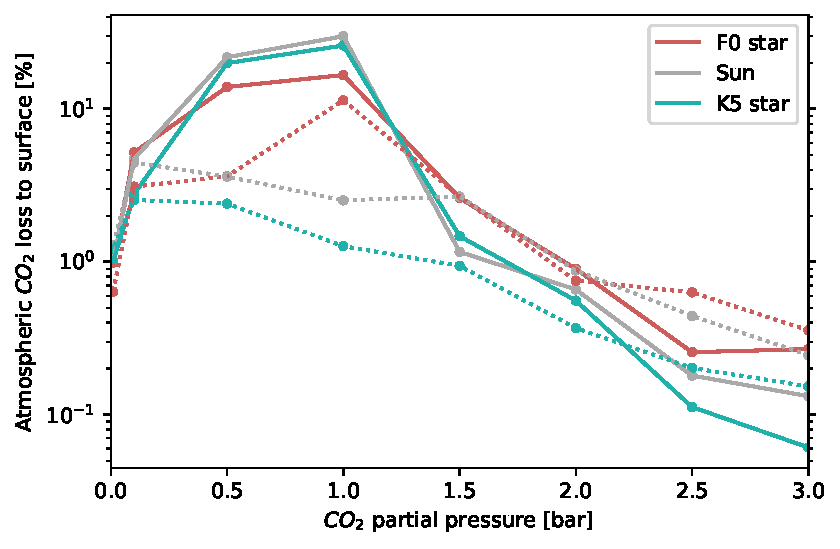
\includegraphics[width=\columnwidth]{Figures/CO2_ice.pdf}
%DIFDELCMD <     %%%
%DIFDELCMD < \caption{%
{%DIFAUXCMD
\DIFdelFL{Global accumulation of $CO_{\mathrm{2}}$ ice for a range of initial atmospheric $CO_{\mathrm{2}}$ pressures for cold start ($T_{\mathrm{surf}}=230$ K) bodies of $0^{\circ}$ (solid lines) and $23.5^{\circ}$ (dashed lines) obliquity orbiting F0, K5, and Sun-like stars at distances of $2.75$, $0.6$, and $1.4$~AU (same orbital distances as in the third row of Figure~\ref{fig:comp_a0}), respectively. The atmospheric $CO_{\mathrm{2}}$ ice loss to surface is defined as the portion of initial $CO_{\mathrm{2}}$ in the atmosphere that precipitates and gets trapped as permanent $CO_{\mathrm{2}}$ ice on the planetary surface.}} %DIFAUXCMD
%DIF < For surface $CO_{\mathrm{2}}$ pressures greater than $1.5$~bar, surface $CO_{\mathrm{2}}$ condensation for all cases becomes negligible.} 
    %DIFDELCMD < 

%DIFDELCMD <     \label{fig:CO2_ice}
%DIFDELCMD < \end{figure}
%DIFDELCMD < 

%DIFDELCMD < %%%
\DIFdelend \section{Discussion}

\subsection{Implications for planetary habitability on early Mars, Earth, and exoplanets}

In agreement with \citet{Turbet2017}, our model \DIFdelbegin \DIFdel{also }\DIFdelend finds that $CO_{\mathrm{2}}$ surface condensation can be a detriment to the habitability of cold start planets (Figure~\ref{fig:ss_all}). As the dense surface $CO_{\mathrm{2}}$ ice becomes sequestered within the subsurface, the atmospheric $CO_{\mathrm{2}}$ pressure decreases, which promotes even more ice formation, possibly leading to atmospheric collapse \citep{Turbet2017}. Unlike Earth, where volcanism ended snowball episodes \citep{Hoffman1342}, it might be more difficult for distant cold planets to avoid permanently glaciated conditions. This is because once $CO_{\mathrm{2}}$ pressures exceed saturation, $CO_{\mathrm{2}}$ is increasingly removed from the atmosphere before temperatures ever become warm enough. An exception to this could be volcanism rich in $H_{\mathrm{2}}$ or $CH_{\mathrm{4}}$, which could produce sufficient $CO_{\mathrm{2}}$-$H_{\mathrm{2}}$ or $CO_{\mathrm{2}}$-$CH_{\mathrm{4}}$ collision-induced absorption at high enough concentrations (percent level) and $CO_{\mathrm{2}}$ pressures \DIFdelbegin \DIFdel{\citep{ramirez2014,ramirez2017,ramirezkalt2018}}\DIFdelend \DIFaddbegin \DIFadd{\citep{ramirez2014,wordsworth_transient_2017,ramirez2017,ramirezkalt2018,turbet_far_2019}}\DIFaddend . Nevertheless, cold start planets that are close enough to their stars receive enough energy to circumvent the above problems (Figure~\ref{fig:ss_all}). 

The above \DIFdelbegin \DIFdel{has }\DIFdelend \DIFaddbegin \DIFadd{provides }\DIFaddend a couple of interesting implications. Some studies argue that Mars (located at $1.52$~AU) was a cold planet that had undergone numerous transient warming episodes over geologic timescales, possibly aided by supplementary volcanic gases or other mechanisms in a predominantly $CO_{\mathrm{2}}$ atmosphere \DIFdelbegin \DIFdel{\citep{wordsworth2013,batalha2016}}\DIFdelend \DIFaddbegin \DIFadd{\citep{wordsworth2013,batalha2016,wordsworth_transient_2017,kite_methane_2020,hayworth_warming_2020}}\DIFaddend . However, multiple sporadic warming episodes would be very difficult to achieve in practice because the excess $CO_{\mathrm{2}}$ will be removed from the atmosphere once a warm period ends. This will not only enhance the ice-albedo feedback, raising the planetary albedo and triggering atmospheric collapse, but the atmospheric $CO_{\mathrm{2}}$ would be gradually removed from the atmospheric-surface system forever as it sinks below the less dense $H_{\mathrm{2}}O$ ice\DIFdelbegin \DIFdel{, making }\DIFdelend \DIFaddbegin \DIFadd{. Some estimates of the early water inventory suggest that early Mars could have had a global equivalent water layer that was at least a couple of hundred meters deep \citep{villanueva2015,ramirezetal2020}.  This would have been a sufficiently large reservoir to absorb much of the condensing surface $CO_{\mathrm{2}}$, decreasing the likelihood of }\DIFaddend subsequent transient warming episodes \DIFdelbegin \DIFdel{much less likely. }\DIFdelend \DIFaddbegin \DIFadd{\citep{Turbet2017}. 
}\DIFaddend 

\DIFaddbegin \DIFadd{In the case of limit cycles for instance (see Methods), models often assume dirty low albedo (0.35) surface $CO_{\mathrm{2}}$ ice \citep{batalha2016, kadoya_outer_2019,hayworth_warming_2020}. This helps reduce the absorbed stellar flux and increases the likelihood of limit cycles. However, observations suggest that the mean $CO_{\mathrm{2}}$ ice albedo on present Mars is much higher \citep{forget2013}. So, assuming such a low albedo on a global scale may be unrealistic. Also, limit cycle models almost always assume a linear relationship between weathering rate and dissolution of H+ in groundwater \citep{batalha2016,kadoya_outer_2019,hayworth_warming_2020}. However, experiments have shown that this relationship is much weaker for real silicate rocks \citep{asolekar1991}, greatly reducing the occurrence of limit cycles \citep{ramirez2017mars}. Thus, it is not clear if such global episodic warm episodes had ever occurred on early Mars, at least during the climate optimum of maximum fluvial incision. If they did, they may have been very few in number.  
}

\DIFaddend In contrast to our cold start cases, our warm start simulations suggest that the condensation of surface $CO_{\mathrm{2}}$ ice affects a much smaller range of orbital distances. Irrespective of the star type, the range of semi-major axes and $CO_{\mathrm{2}}$ pressures for which planets exhibit habitable surface conditions is similar to that predicted by 1-D calculations of the habitable zone \citep{kasting1993, Ramirez2018}. That said, warm start cases that are distant enough to \DIFdelbegin \DIFdel{exhibit significant }\DIFdelend \DIFaddbegin \DIFadd{manifest significant surface }\DIFaddend $CO_{\mathrm{2}}$ condensation suffer the same habitability problems discussed above for cold start planets. 

These results also have implications for our own planet. The Earth, by definition, is located close enough to the star where surface $CO_{\mathrm{2}}$ ice condensation is impossible under normal circumstances (Figure~\ref{fig:ss_all}), and it would have been warm so long as the greenhouse effect, including from $CO_{\mathrm{2}}$, was potent enough. Nevertheless, the Hadean Earth likely had a $CO_{\mathrm{2}}$-rich atmosphere \citep{kasting2014}, suggesting that it was almost certainly a warm start planet, \DIFdelbegin \DIFdel{which may have possibly helped facilitate }\DIFdelend \DIFaddbegin \DIFadd{possibly facilitating }\DIFaddend an early emergence of life.

\subsection{Comparison with previous \DIFdelbegin \DIFdel{work}\DIFdelend \DIFaddbegin \DIFadd{studies}\DIFaddend }
\DIFaddbegin 

\DIFaddend Although we obtain similar trends, our cold start results differ in certain respects from those of \citet{Turbet2017}. In particular, there are discrepancies in the spatial coverage of \DIFdelbegin \DIFdel{red (warm }\DIFdelend \DIFaddbegin \DIFadd{the red (ice-free or partially ice-covered }\DIFaddend planets) and blue (cold and icy \DIFaddbegin \DIFadd{planets }\DIFaddend displaying surface $CO_{\mathrm{2}}$ ice) colored \DIFdelbegin \DIFdel{areas }\DIFdelend \DIFaddbegin \DIFadd{regions }\DIFaddend in Figure~\ref{fig:ss_all} between the two studies, which are likely to be mostly attributed to model differences (although there are slight differences in definition of the regions also). In particular, EBMs \DIFdelbegin \DIFdel{, }\DIFdelend such as this one \DIFdelbegin \DIFdel{, }\DIFdelend are quite sensitive to the ice-albedo feedback, and are thus more prone to abrupt transitions between cold and warm climate states \citep{RamirezLevi2018}. Our model also employs an atmospheric-ocean heat transport parameterization which likely produces different model behavior \DIFdelbegin \DIFdel{than }\DIFdelend \DIFaddbegin \DIFadd{during the transition between icy and warm climates than what }\DIFaddend the static ocean assumption \DIFdelbegin \DIFdel{made in \citet{Turbet2017} . 
}\DIFdelend \DIFaddbegin \DIFadd{of \citet{Turbet2017} would yield. It is unclear how GCMs with fully-coupled atmospheric oceans may compare with the results presented here. This would be an interesting consideration for future studies. 
}\DIFaddend 

\DIFdelbegin \DIFdel{Another }\DIFdelend \DIFaddbegin \DIFadd{We note that at low $CO_{\rm 2}$ partial pressures surface $CO_{\rm 2}$ condensation is more easily reached than what is qualitatively shown in Figure~\ref{fig:Sketch}. However, when planets are located far away enough from the host star and/or surface temperatures are low enough (such as for cold starts), $CO_{\rm 2}$ condensation can easily take place during the evolution of the planet, once saturation pressure is reached. Some of the difference may be due to $H_{\rm 2}O$ ice cloud warming that some GCMs predict in dry and cold atmospheres, but our model does not. An alternative }\DIFaddend reason for the differences may be in the \DIFdelbegin \DIFdel{treatment of clouds. For instance, our }\DIFdelend \DIFaddbegin \DIFadd{spatial and vertical distributions of clouds, which are not accurately predicted by EBMs. Furthermore, the }\DIFaddend $CO_{\mathrm{2}}$ clouds \DIFdelbegin \DIFdel{impact }\DIFdelend \DIFaddbegin \DIFadd{formed in our simulations impact the }\DIFaddend planetary albedo, but they are non-absorbing (see \DIFdelbegin \DIFdel{Methods}\DIFdelend \DIFaddbegin \DIFadd{Section~\ref{sec:Methods}}\DIFaddend ). In contrast, the $CO_{\mathrm{2}}$ clouds of \citet{Turbet2017} are either radiatively active or inactive across the entire spectrum. Nevertheless, other GCM results are consistent with 1-D results (and, in turn, the EBM results here \DIFdelbegin \DIFdel{) }\DIFdelend in the location of the outer edge of the habitable zone\DIFdelbegin \DIFdel{\citep{wolf2018erratum}.
Also, our }\DIFdelend \DIFaddbegin \DIFadd{; \citet{wolf2018erratum}).
Our }\DIFaddend warm start results agree well with those predicted from 1-D radiative-convective climate models \citep{kasting1993, KumarKopparapu2013, Ramirez2018}.
\DIFdelbegin \DIFdel{However, it is unclear how GCMs with fully-coupled atmospheric oceans may compare with the results here. This would be an interesting consideration for future studies. }\DIFdelend 

\DIFaddbegin \DIFadd{Surface condensation of $CO_{\mathrm{2}}$ ice is highly dependent on the equator-to-pole temperature contrast, which in turn is sensitive to the diffusion coefficient $D$ (Equation~\ref{hdiff}), which includes the planetary obliquity. We compared our results with those of past GCM simulations of snowball planets \citep{hoffman_snowball_2017} to test the reliability of our diffusion parameterization. Figure~\ref{fig:Hoffman_comparison} shows the predicted latitudinally-averaged surface temperature distributions in our model. In general, our results agree quite well with the ones of \citet{hoffman_snowball_2017}, lying near the lower range of surface temperatures, similar to the FOAM (Fast Ocean Atmosphere Model) model. Some of the GCM simulations are slightly warmer than ours (except for the FOAM model) because they predict the formation of highly-absorbing upper atmospheric $H_{\rm 2}O$ ice clouds in these cold and (otherwise) dry atmospheres. More models should test this result. Nevertheless, we conclude that our employed heat diffusion parameterization is reasonable and consistent with previous studies.
}

\begin{figure}
	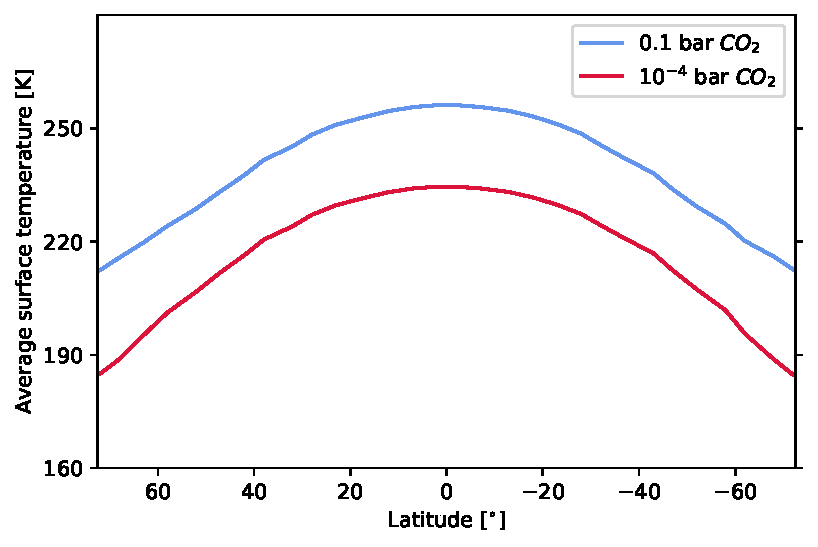
\includegraphics[width=\columnwidth]{Figures/Hoffman_comparison.pdf}
    \caption{\DIFaddFL{Average surface temperature as a function of latitude obtained using initial conditions corresponding to the GCM by \citet{hoffman_snowball_2017} (Figure 8a), for initial atmospheric $CO_{\rm 2}$ contents of $0.11$~mbar and $100$~mbar. The surface albedo was set to $0.6$ everywhere while planetary obliquity and eccentricity were set to $23.5^{\circ}$, and zero, respectively.}}
    \label{fig:Hoffman_comparison}
\end{figure}

\DIFadd{In summary, the main differences between EBMs and GCMs are mainly related to how large scale dynamics (which might lead to sharper climatic transitions) and clouds are treated, whose spatial and vertical distributions cannot be accurately predicted by EBMs. Nevertheless, EBMs are computationally efficient,  enabling exploration of a wide parameter space, which would be computational expensive with GCMs. Furthermore, since this study mainly addresses different climatic trends and distributions, EBMs such as this one are appropriate tools. 
Nevertheless, improved observations are needed to test how well climate models, irrespective of complexity, agree with reality.
}

\DIFaddend \section{Conclusions}
%DIF <  The last numbered section should briefly summarise what has been done, and describe the final conclusions which the authors draw from their work.
Planets similar to Earth might experience cold or warm stages during the course of their evolution. The carbonate-silicate cycle can stabilize planetary temperatures over geological timescales. While  $CO_{\mathrm{2}}$ generally increases surface temperature, high enough atmospheric $CO_{\mathrm{2}}$ can trigger atmospheric collapse via $CO_{\mathrm{2}}$ surface ice condensation (starting at the poles), leading to irreversible glaciation. Such a process could negatively impact the habitability of terrestrial bodies, even if located within the canonical habitable zone. This was argued in \citet{Turbet2017}, whom showed that surface $CO_{\mathrm{2}}$ ice condensation on initially frozen planets orbiting the Sun can significantly reduce the range of habitable orbital distances. 

Our work here confirms these results and extends the analysis to rapidly-rotating planets under different starting temperature conditions orbiting a range of star types (F - K). Using a latitudinally-dependent EBM, we show that planets that start out warm \DIFdelbegin \DIFdel{can delay }\DIFdelend \DIFaddbegin \DIFadd{generally exhibit }\DIFaddend surface $CO_{\mathrm{2}}$ ice condensation \DIFdelbegin \DIFdel{to significantly higher $CO_{\mathrm{2}}$ pressures and }\DIFdelend \DIFaddbegin \DIFadd{at significantly }\DIFaddend larger orbital distances than \DIFdelbegin \DIFdel{can }\DIFdelend cold start (i.e., fully glaciated with $T_{\mathrm{surf}}=230$~K) planets. This implies a wide habitable zone, consistent with what had been previously computed using simpler 1-D models \citep{kasting1993,KumarKopparapu2013,Ramirez2018}. Although our model predicts that this zone remains similarly wide across obliquities, we find that inefficient poleward heat transport leads to more surface  $CO_{\mathrm{2}}$ ice production at lower ($0^{\circ}$) obliquity. \DIFaddbegin \DIFadd{Finally, our heat diffusion parameterization provides a simple way of evaluating a range of warm and cold climates with minimal tuning of parameters. 
}\DIFaddend 

The physics of planetary atmospheres \DIFdelbegin \DIFdel{remains }\DIFdelend \DIFaddbegin \DIFadd{remain }\DIFaddend complex, particularly for planets unlike the Earth. Future work should continue to use a hierarchy of models to explore the \DIFdelbegin \DIFdel{effect }\DIFdelend \DIFaddbegin \DIFadd{effects }\DIFaddend of clouds, convection, and the impact that oceans have on the overall heat transport. 

\section*{Acknowledgements}
I.B. acknowledges financial support from the Japanese Ministry of Education, Culture, Sports, Science and Technology (MEXT).
R.M.R. acknowledges funding from the Earth-Life Science Institute (ELSI) and from the National Institutes of Natural Sciences: Astrobiology Center (grant number JY310064).
\DIFdelbegin %DIFDELCMD < 

%DIFDELCMD < %%%
%DIF <  \begin{figure*}
%DIF <  	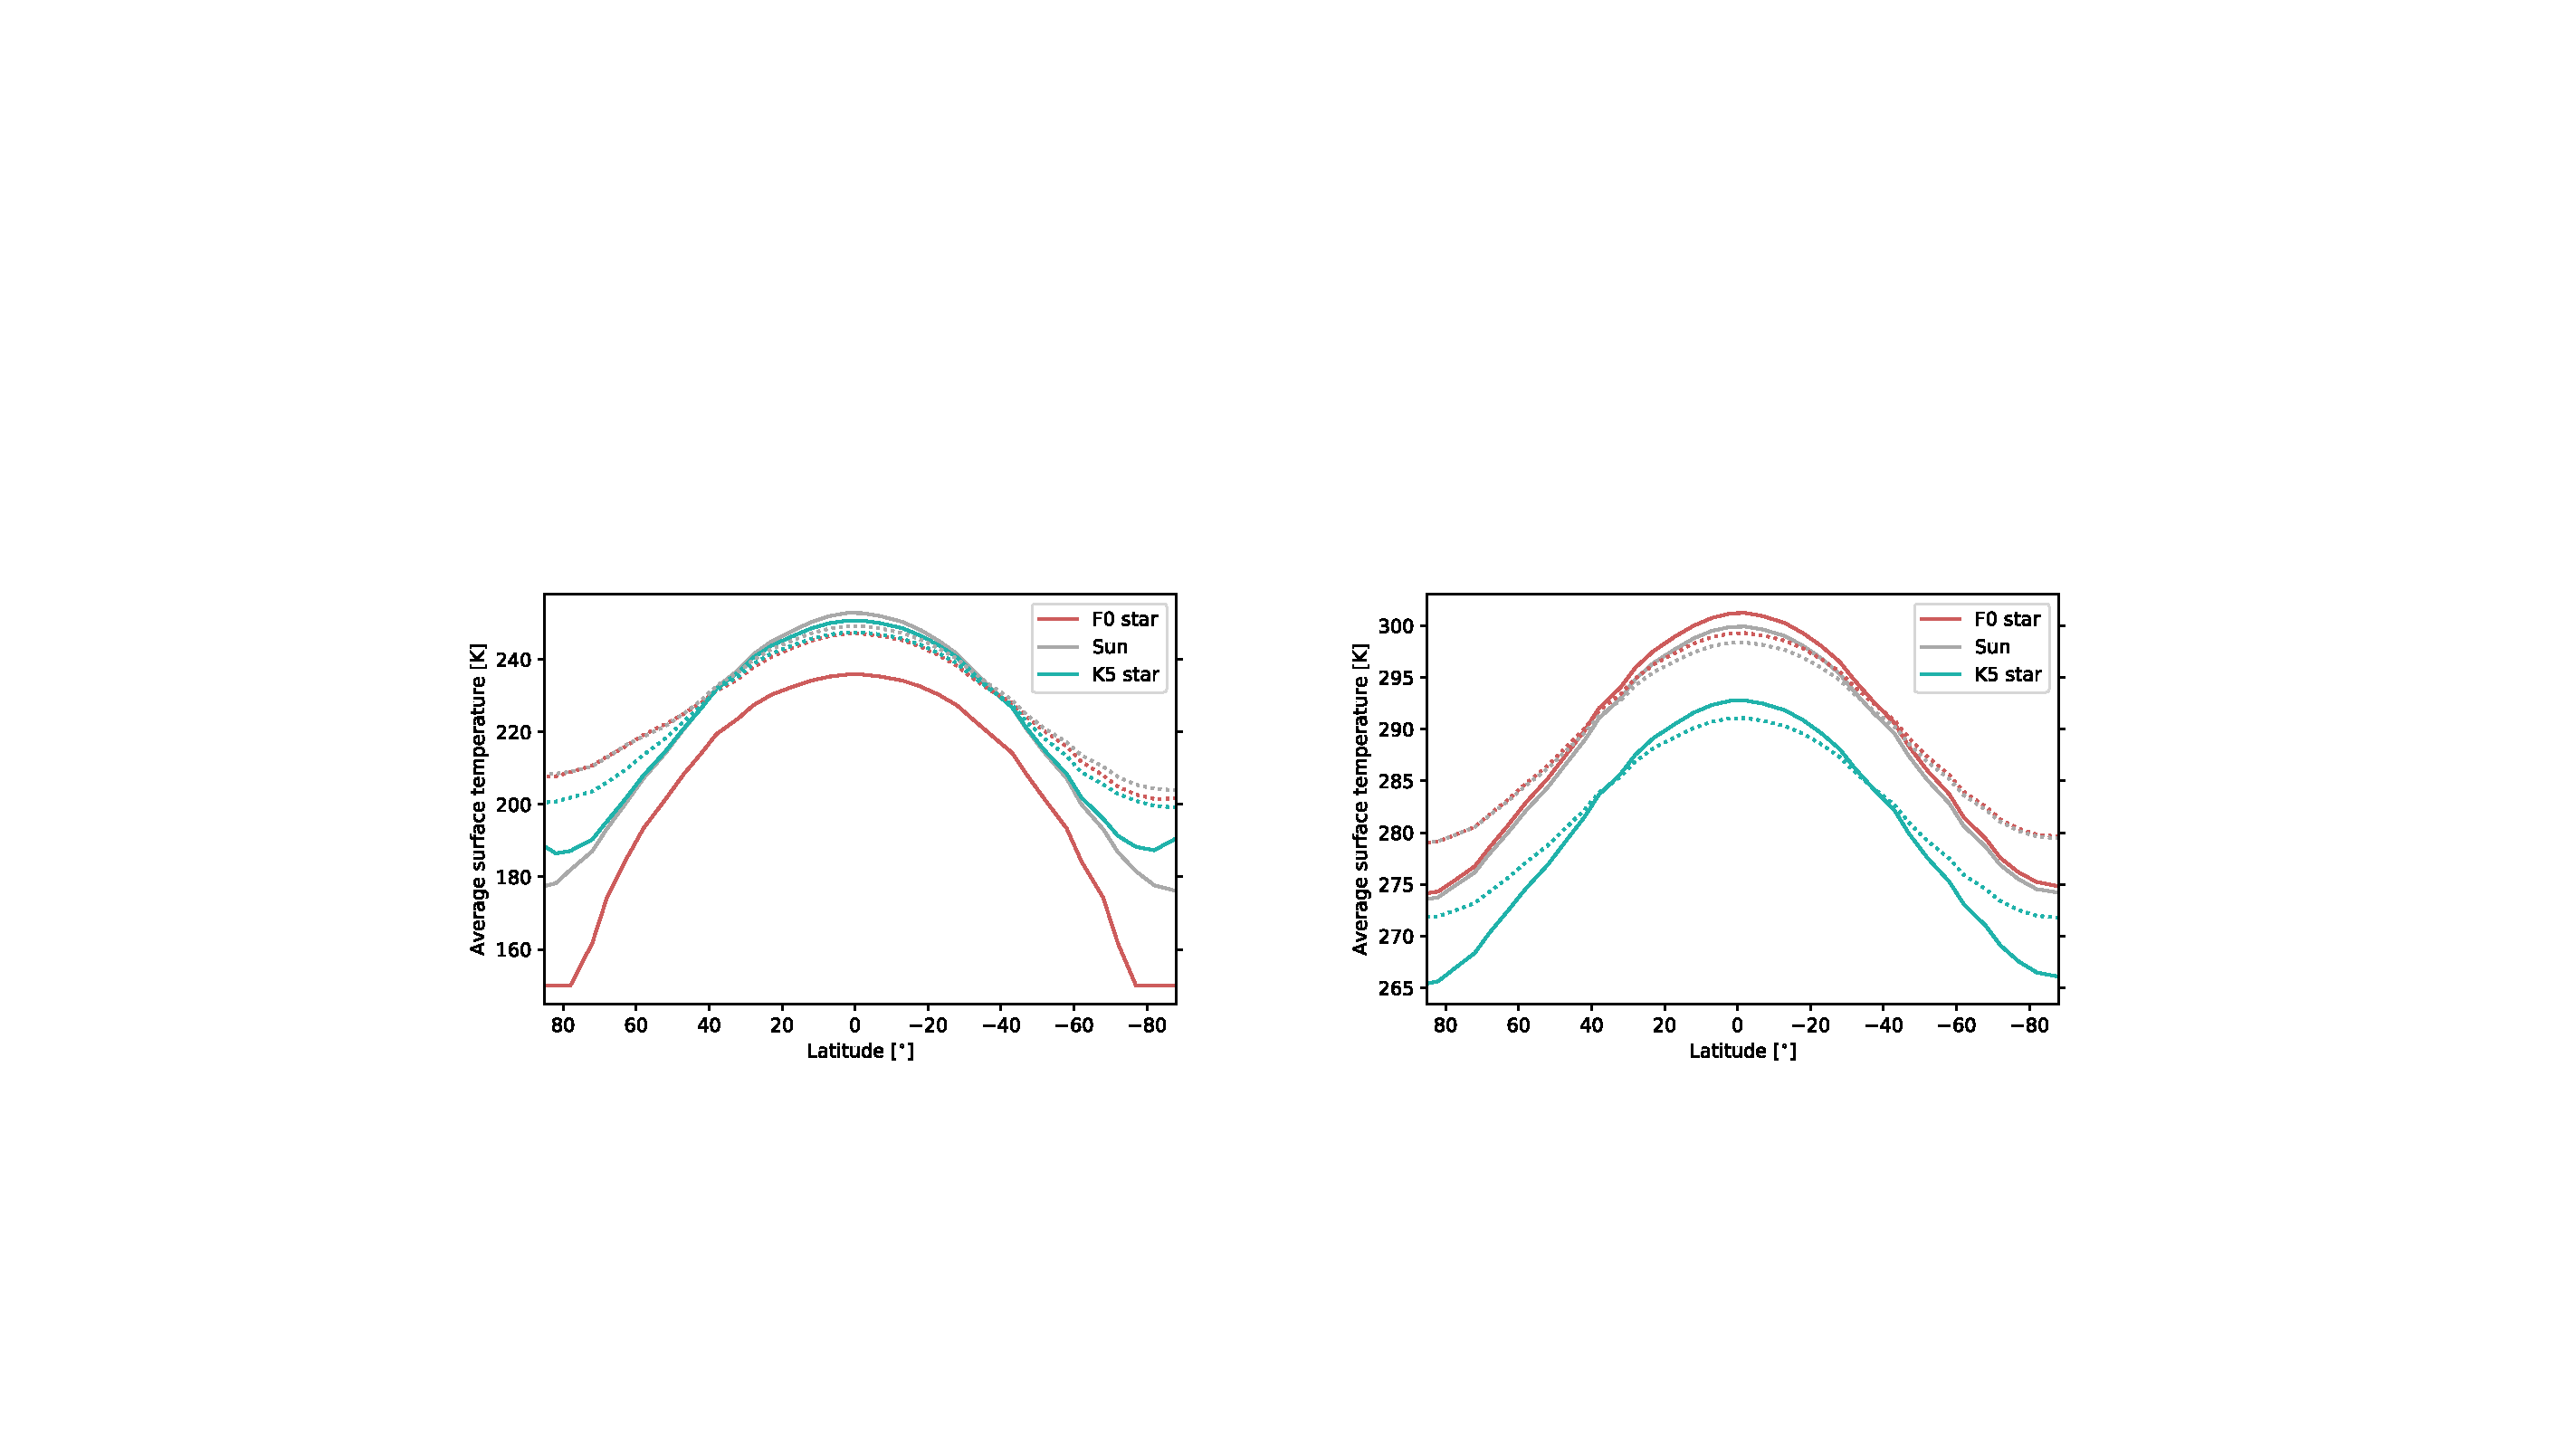
\includegraphics[width=\textwidth]{Figures/Comparison_Tsurf.pdf}
%DIF <      \caption{Average surface temperature at the last time step as a function of latitude for cold start ($T_{\mathrm{surf}}=230$~K) and warm start ($T_{\mathrm{surf}}=230$~K) bodies having an initial atmospheric $CO_{\mathrm{2}}$ pressure of $1$~bar and obliquities $0^{\circ}$ (solid lines) and $23.5^{\circ}$ (dashed lines). The colors indicate planets orbiting F0, K5, and Sun-like stars at distances of $2.4$, $0.55$, and $1.25$~AU, respectively.}
%DIF <      \label{fig:comp_T_ave}
%DIF <  \end{figure*}
\DIFdelend 

%%%%%%%%%%%%%%%%%%%%%%%%%%%%%%%%%%%%%%%%%%%%%%%%%%

%%%%%%%%%%%%%%%%%%%% REFERENCES %%%%%%%%%%%%%%%%%%

% The best way to enter references is to use BibTeX:

\bibliographystyle{mnras}
\bibliography{bibliography} % if your bibtex file is called example.bib


% Alternatively you could enter them by hand, like this:
% This method is tedious and prone to error if you have lots of references
%\begin{thebibliography}{99}
%\bibitem[\protect\citeauthoryear{Author}{2012}]{Author2012}
%Author A.~N., 2013, Journal of Improbable Astronomy, 1, 1
%\bibitem[\protect\citeauthoryear{Others}{2013}]{Others2013}
%Others S., 2012, Journal of Interesting Stuff, 17, 198
%\end{thebibliography}

%%%%%%%%%%%%%%%%%%%%%%%%%%%%%%%%%%%%%%%%%%%%%%%%%%

%%%%%%%%%%%%%%%%% APPENDICES %%%%%%%%%%%%%%%%%%%%%

%\appendix

%\section{Some extra material}

%%%%%%%%%%%%%%%%%%%%%%%%%%%%%%%%%%%%%%%%%%%%%%%%%%


% Don't change these lines
\bsp	% typesetting comment
\label{lastpage}
\end{document}

% End of mnras_template.tex